\documentclass[12pt]{article}
\usepackage[hidelinks]{hyperref}
\newtheorem{theorem}{Theorem}
\usepackage{import}
\usepackage{mathtools}
\usepackage{xcolor}
\usepackage{textcomp}
\usepackage[italian]{babel}
\usepackage{graphicx}
\usepackage{outlines}
\AddToHook{cmd/section/before}{\clearpage} 
\newcommand{\circumdelta}{%
  \leavevmode\vbox{
    \offinterlineskip
    \ialign{%
      \hfil##\hfil\cr
      \^{}\cr\noalign{\vskip-1ex}
      $\delta$\cr
    }
  }%
}

\begin{document}
\tableofcontents
\newpage

\section{Introduzione}
\subsection{Motivazione}
Un linguaggio è uno strumento per descrivere come risolvere i problemi in maniera rigorosa, in modo tale che sia eseguibile da un calcolatore
Perché è utile studiare come creare un linguaggio di programmazione?
\begin{itemize}
	\item non rimanere degli utilizzatori passivi
	\item capire il funzionamento dietro le quinte di un linguaggio
	\item domain-specific language (DSL): è un linguaggio pensato per uno specifico problema
	\item model drivern software development: modo complesso per dire UML e simili
	\item model checking
\end{itemize}


\subsection{Definizioni base}
Un linguaggio è composto da:
\begin{itemize}
	\item lessico e sintassi
	\item compilatore: parser + generatore di codice oggetto
\end{itemize}
La generazione automatica di codice può essere dichiarativa lessico
(espressioni regolari o automa a stati finite) o sintassi(grammatiche o automa a pile).
Un automa a stati finiti consuma informazioni una alla volta, ne salva una quantità finita. Alcuni esempi di applicazione di automa a stati finiti: software di progettazione di circuiti, analizzatore lessicale, ricerca di parole sul web e protocolli di comunicazione.

\begin{figure}[ht]
	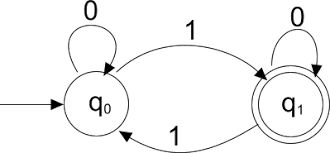
\includegraphics[scale = 0.3]{media/semplice_automa.png}
	\centering
	\caption{Semplice automa}
\end{figure}

\subsection{Contenuti del corso}
\begin{outline}
	\1 Linguaggi formali e Automi:
	\2 Automi a stati finiti, espressioni regolari, grammatiche libere, automi a pila, Macchine di Turing, calcolabilità
	\1 Compilatori:
	\2 Analisi lessicale, analisi sintattica, analisi semantica, generazione di codice
	\1 Logica di base:
	\2 Logica delle proposizioni e dei predicati
	\1 Modelli computazionali:
	\2 Specifica di sistemi tramite sistemi di transizione, logiche temporali per la specifica e verifica di proprietà dei sistemi (model checking), sistemi concorrenti (algebre di processi e reti di Petri)
\end{outline}

\subsection{Informazioni utili}
Parte integrante del corso:
\begin{outline}
	\1 Supporto alla parte teorica usando tool specifici.
	\2 JFLAP 7.1: http://www.jflap.org (automi/grammatiche)
	\2 Tina 3.7.5: http://projects.laas.fr/tina
	(model checking di sistemi di transizione e reti di Petri)
	\2 LTSA 3.0: http://www.doc.ic.ac.uk/ltsa
	(sistemi di transizione definiti tramite algebre di processi)
	\1 Nel resto del corso utilizzeremo un ambiente di sviluppo per
	generare parser/compilatori
	\2 IntelliJ esteso con plug-in ANTLRv4, ultima versione 1.20
	(generatore ANTLR: http://www.antlr.org/)
\end{outline}

\newpage
Libri di testo suggeriti:
\begin{outline}
	\1 J. E. Hopcroft, R. Motwani e J. D. Ullman:
	Automi, linguaggi e calcolabilita’,
	Addison-Wesley, Terza Edizione, 2009. Cap. 1–9
	\1 A. V. Aho, M. S. Lam, R. Sethi e J. D. Ullman:
	Compilatori: principi tecniche e strumenti,
	Addison Wesley, Seconda Edizione, 2009. Cap. 1–5
	\1 M. Huth e M. Ryan:
	Logic in Computer Science: Modelling and Reasoning about
	Systems,
	Cambridge University Press, Second Edition, 2004. Cap. 1–3
\end{outline}

\section{Linguaggi regolari}
\subsection{Alfabeti}
Un \emph{alfabeto} è un insieme finito e non vuoto di simboli, comunemente indicato con $\Sigma$. Seguono alcuni esempi di alfabeti:
\begin{outline}
	\1 $\Sigma$ = \{0,1\} alfabeto binario
	\1 $\Sigma$ = \{a,b,...,z\} alfabeto di tutte lettere minuscole
	\1 L'insieme ASCII
\end{outline}

\subsubsection{Stringhe}
Una stringa/parola è un insieme di simboli di un alfabeto, 0010 è una stringa che appartiene $\Sigma$ = \{0,1\}.
\\ La \emph{stringa vuota} è una stringa composta da 0 simboli.
\\ La lunghezza della stringa sono il numeri di caratteri che la compongono (non devono essere unici). La sintassi per la lunghezza di una stringa w è $|w|$, quindi $|001|$ = 3 oppure $|\epsilon| = 0$ (nota bene, $\epsilon \ne 0$ ma è di lunghezza 0).

\subsubsection*{Potenze di un alfabeto}
Se $\Sigma$ è un alfabeto si può esprimere l'insieme di tutte le stringhe di una certa lunghezza con una notazione esponenziale: $\Sigma^k$ denota tutte le stringhe di lunghezza k con simboli che appartengono a $\Sigma$. \\
Per esempio:
\\ $\Sigma^1$ = \{0,1\}
\\ $\Sigma^2$ = \{00, 01, 10, 11\}
\\ $\Sigma^2$ = \{000, 001, 010, 011, 100, 101, 110, 111\}
\\ L'insieme delle stringhe meno quella vuota è segnato come $\Sigma^+$, mentre l'insieme che include la stringa vuota è $\Sigma^*$,

\subsubsection{Concatenazione di stringhe}
Siano x e y stringhe, dove i è la lunghezza di x e j è la lunghezza di y, la stringa xy è la stringa risultata dalla concatenazione delle stringhe xy di lunghezza i+j.

\subsection{Definizione di linguaggio}
Un insieme di stringhe a scelta L $\subseteq\Sigma^*$ si definisce linguaggio su $\Sigma$.
\\ Un modo formale per definire un alfabeto è il seguente \{w $|$ enunciato su w\}, che si traduce in "w tale che enunciato su w".
\\ $\{0^n 1^n | n \ge 1 \}$ si traduce in "l’insieme di 0 elevato alla n, 1 alla n tale che n è maggiore o uguale a 1"

\section{Automa a stati finiti deterministico}
Un automa a stati finiti deterministico consiste in:
\begin{enumerate}
	\item Un insieme di stati finiti Q
	\item Un insieme di simboli di input, $\Sigma$
	\item Una funzione di transizione, che prende in input uno stato e un simbolo e restituisce uno stato. Tale funzione è spesso indicato con $\delta$ ed è usata per rappresentare i archi nella rappresentazione grafica. Ovvero sia \emph{q} uno stato, \emph{a} un input allora $\delta$(q,a) è lo stato \emph{p} tale che esista un arco da q a p.
	\item Uno stato iniziale (naturalmente che appartiene a Q)
	\item Un insieme di stati accettati finali F. Questo è un sottoinsieme di Q.
\end{enumerate}
Un automa a stati finiti deterministico è spesso chiamato con l'acronimo DFA e viene può essere rappresentato nella seguente maniera concisa:
\[A = (Q, \Sigma, \delta, q\textsubscript{0}, F)\]
Dove A rappresenta il DFA.

\subsection{ Elaborazione di stringhe }
Per elaborare una stringa è si definisce lo stato iniziale, quello finale e una serie di regole di transizione per poterci arrivare.
Se dovessi decodificare la stringa 01 il DFA risulterebbe:
\[A = (Q=\{q1,q2,q3\}, \{0,1\}, \delta, q\textsubscript{0}, \{q1\})\]
I stati sono i sequenti:
\\ $\delta(q\textsubscript{0},1)=q\textsubscript{0}$: leggo come primo stato 1, nessun progresso fatto
\\ $\delta(q\textsubscript{0},0)=q\textsubscript{2}$: leggo come primo stato 0, posso andare avanti e cercare un 1
\\ $\delta(q\textsubscript{2},1)=q\textsubscript{1}$: leggo 1 dopo lo 0, ho trovato la stringa
\\ $\delta(q\textsubscript{2},0)=q\textsubscript{2}$: leggo 0 dopo lo 0, non ho fatto progresso
\\ Nota bene: questa è una notazione arbitraria del libro, q1 e q2 si possono invertire.

\subsubsection{ Notazioni semplici per DFA }
\subsubsection*{ Diagramma di transizione }
Dato un DFA $A = (Q, \Sigma, \delta, q\textsubscript{0}, F)$ un suo diagramma di transizione è composto da:
\begin{outline}
	\1 Ogni stato Q è un nodo
	\1 Ogni funzione $\delta$ è una freccia
	\1 La freccia Start che denota il primo input
	\1 Gli stati accettati F hanno un doppio cerchio
\end{outline}
\begin{figure}[ht]
	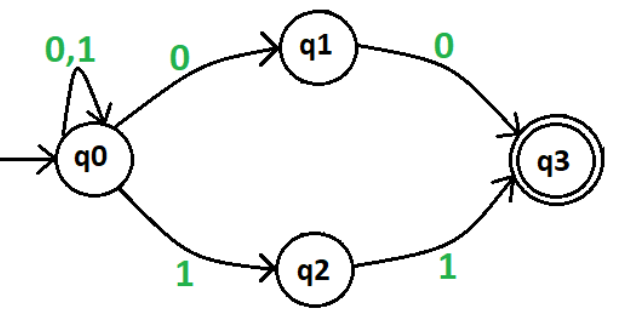
\includegraphics[scale = 0.3]{media/diagramma_stato.png}
	\centering
	\caption{Diagramma di transizione}
\end{figure}

\subsubsection*{ Tabelle di transizione }
Una tabella di transizione è costituita nelle riga dalle funzioni $\delta$ e nelle colonne dagli input. Ogni incrocio equivale a uno stato della funzione $\delta$ con un input generico \emph{a}.

\begin{table}[ht]
	\centering
	\begin{tabular}{c | c | c}
		                                  & 0                  & 1                  \\
		\hline
		$\rightarrow$  q\textsubscript{0} & q\textsubscript{2} & q\textsubscript{0} \\
		$*$q\textsubscript{1}             & q\textsubscript{1} & q\textsubscript{1} \\
		q\textsubscript{2}                & q\textsubscript{2} & q\textsubscript{1} \\
	\end{tabular}
	\caption{Esempio di tabella}
\end{table}

La freccia è lo start e l'asterisco è lo stato finale.

\subsubsection{ Estensione della funzione di transizione di stringhe }
Allo scopo di poter seguire una sequenza di input ci serve definire una funzione di transizione estesa. Se $\delta$ è una funzione di transizione, chiameremo \circumdelta\space la sua funzione estesa.
La funzione estesa prende in input \emph{q} e una stringa \emph{w} e ritorna uno stato \emph{p}.
\\ Ogni stato viene calcolato grazie allo stato esteso precedente: \[\circumdelta(\emph{q,w}) = \delta(\circumdelta(\emph{q,x}), \emph{a})\]
\subsubsection*{Esempio}
L = \{ \emph{w} $|$ \emph{w} ha un numero pari di 0 e di 1 \}
\\ Nota bene: 0 (numero di simboli) è pari quindi conta come stato accettato, ed è l'unico stato accettato.
\\ \hspace*{0.4cm} q\textsubscript{0}: 0 e 1 sono pari
\\ \hspace*{0.4cm} q\textsubscript{1}: 0 pari 1 dispari
\\ \hspace*{0.4cm} q\textsubscript{2}: 1 pari 0 dispari
\\ \hspace*{0.4cm} q\textsubscript{3}: 0 dispari 1 dispari
\[A = (\{q0,q1,q2,q3\}, \{0,1\}, \delta, q\textsubscript{0}, \{q\textsubscript{0}\})\]

\begin{figure}[ht]
	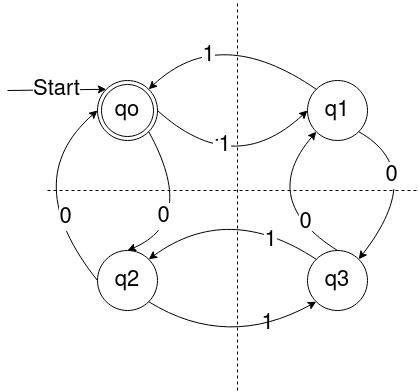
\includegraphics[scale = 0.5]{media/stringhe_pari.png}
	\centering
	\caption{Diagramma}
\end{figure}

\begin{table}[ht]
	\centering
	\begin{tabular}{c | c | c}
		                                   & 0                  & 1                  \\
		\hline
		$\rightarrow *$ q\textsubscript{0} & q\textsubscript{2} & q\textsubscript{1} \\
		q\textsubscript{1}                 & q\textsubscript{3} & q\textsubscript{0} \\
		q\textsubscript{2}                 & q\textsubscript{0} & q\textsubscript{3} \\
		q\textsubscript{3}                 & q\textsubscript{1} & q\textsubscript{2} \\
	\end{tabular}
	\caption{Esempio funzioni}
\end{table}

\newpage
Ora applichiamo le funzione di transizione estesa per verificare che 110101 abbia 0 e 1 pari:
\begin{itemize}
	\item  \circumdelta$(q\textsubscript{0}, \epsilon)$ = q\textsubscript{0}
	\item  \circumdelta$(q\textsubscript{0}, 1)$ = $\delta(\circumdelta(q\textsubscript{0}, \epsilon),1)$ = $\delta(q\textsubscript{0},1)$ =  q\textsubscript{1}
	\item  \circumdelta$(q\textsubscript{0}, 11)$ = $\delta(\circumdelta(q\textsubscript{0}, 1),1)$ = $\delta(q\textsubscript{1},1)$ =  q\textsubscript{0}
	\item  \circumdelta$(q\textsubscript{0}, 110)$ = $\delta(\circumdelta(q\textsubscript{1}, 11),0)$ = $\delta(q\textsubscript{0},1)$ =  q\textsubscript{2}
	\item  \circumdelta$(q\textsubscript{0}, 1101)$ = $\delta(\circumdelta(q\textsubscript{0}, 110),1)$ = $\delta(q\textsubscript{2},1)$ =  q\textsubscript{3}
	\item  \circumdelta$(q\textsubscript{0}, 11010)$ = $\delta(\circumdelta(q\textsubscript{0}, 1101),0)$ = $\delta(q\textsubscript{3},0)$ =  q\textsubscript{1}
	\item  \circumdelta$(q\textsubscript{0}, 110101)$ = $\delta(\circumdelta(q\textsubscript{0}, 11010),1)$ = $\delta(q\textsubscript{1},1)$ =  q\textsubscript{0}

\end{itemize}
A ogni simbolo aggiunto posso usare la funzione estesa precedente per calcolare il prossimo stato, in questo caso la sequenza ha un numero pari di 0 e 1.

\section{Automa a stati finiti non deterministici}
Un NFA (nondeterministic finite automaton) può trovarsi contemporaneamente in diversi stati. L'automa "scommette" sul input su certe proprietà dell'input.
\\ I NFA sono spesso più succinti e facili da definire rispetto ai DFA, un DFA può avere un numero di stati addirittura esponenziale rispetto a un NFA. Ogni NFA può essere convertito in un DFA.

\newpage
\subsection{Descrizione informale}
A differenza di un DFA, una funzione di stato in un NFA può restituire 0 o più stati. Immaginiamo di dover identificare se una stringa finisce con 01.
\\ Di seguito il diagramma di transizione sarà il seguente.
\begin{figure}[ht]
	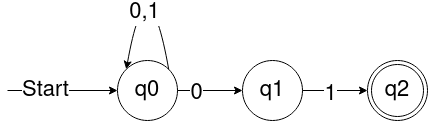
\includegraphics[scale = 0.5]{media/01_end.png}
	\centering
	\caption{NFA che accetta stringa che finisce con 01}
\end{figure}
Come è possibile notare q\textsubscript{0} può può restituire due stati se riceve uno 0. Il NFA esegue molteplici stadi alla ricerca del pattern (simile a un processo che si moltiplica).

\begin{figure}[ht]
	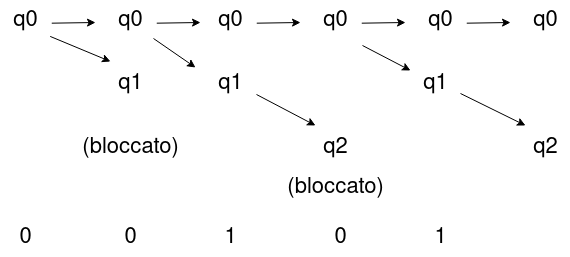
\includegraphics[scale = 0.5]{media/NFA_es.png}
	\centering
	\caption{Gli stati del NFA}
\end{figure}
Ogni volta che il NFA accetta uno stato 0 crea due processi, un q\textsubscript{1} e q\textsubscript{0}
A ogni successivo input tutti i processi vanno avanti, nel nostro caso il q\textsubscript{1} "muore". Al secondo giro viene creato q\textsubscript{1} che muore alla quarta iterazione perché non è l'ultimo simbolo. Durante la quarta iterazione nasce q\textsubscript{1} che alla quinta ci porta uno stato accettato.

\newpage
\subsection{Definizione formale}
Formalmente un NFA si definisce come un DFA.
\[A = (Q, \Sigma, \delta, q\textsubscript{0}, F)\]
\begin{enumerate}
	\item Un insieme di stati finiti Q
	\item Un insieme di simboli di input, $\Sigma$
	\item Una funzione di transizione, che prende in input uno stato e un simbolo e restituisce \emph{\textbf{un insieme di stati}}. Questa è l'unica differenza rispetto al DFA, dove ci viene restituito un singolo stato.
	\item Uno stato iniziale (naturalmente che appartiene a Q)
	\item Un insieme di stati accettati finali F. Questo è un sottoinsieme di Q.
\end{enumerate}

\begin{table}[ht]
	\centering
	\begin{tabular}{c || c | c}
		                                 & 0                                          & 1                      \\
		\hline\hline
		$\rightarrow$ q\textsubscript{0} & \{q\textsubscript{0}, q\textsubscript{1}\} & \{q\textsubscript{0}\} \\
		q\textsubscript{1}               & $\emptyset$                                & \{q\textsubscript{2}\} \\
		$*$q\textsubscript{2}            & $\emptyset$                                & $\emptyset$            \\
	\end{tabular}
	\caption{Tabella di transizione di una NFA che accetta una stringa che finisce con 01}
\end{table}
L'unica differenza con una tabella DFA è che negli incroci ci sono dei insiemi di stati di output (singoletto quanto è uno solo), mentre se la transizione non esiste viene segnata con $\emptyset$.

\newpage
\subsection{Funzione di transizione estesa}
Come per i DFA bisogna prendere la funzione di transizione e renderla estesa. In questo caso lo stato precedente può ritorna un insieme di stati, quindi bisognare fare l'unione di questi. La funzione estesa di $\delta$ si chiamerà \circumdelta.
\[\bigcup^k_{x=2}\delta(p_i,a) = \{r_1,r_2,... ,r_m\} \]
Usiamo \circumdelta\space per calcolare se la stringa 00101 finisce con 01.

\begin{enumerate}
	\item $\circumdelta(q_0, \epsilon) = \{q_0\}$
	\item $\circumdelta(q_0, 0) = \delta(q_0,0) = \{q_0, q_1\}$
	\item $\circumdelta(q_0, 00) = \delta(q_0,0) \cup \delta(q_1,0)  = \{q_0, q_1\} \cup \emptyset = \{q_0, q_1\} $
	\item $\circumdelta(q_0, 001) = \delta(q_0,1) \cup \delta(q_1, 1) = \{q_0\} \cup \{q_2\} = \{q_0, q_2\}$
	\item $\circumdelta(q_0, 0010) = \delta(q_0,0) \cup \delta(q_2, 0) = \{q_0, q_1\} \cup \emptyset = \{q_0, q_1\}$
	\item $\circumdelta(q_0, 00101) = \delta(q_0,1) \cup \delta(q_1, 1) = \{q_0\} \cup \{q_2\} = \{q_0, q_2\}$
\end{enumerate}
Abbiamo un risultato positivo, $q_2$ mentre $q_0$ viene scartato

\subsection{Linguaggio NFA}
Come abbiamo visto sopra, il fatto di avere uno stato non accettabile al termine dell'operazione non significa che non abbia avuto successo.
\\ Formalmente se $A = (Q, \Sigma, \delta, q\textsubscript{0}, F)$ è un NFA allora:
\[L(A) = \{ w | \circumdelta(q_0, w) \cap \emph{F} \ne \emptyset \}\]
In parole povere L(A) è l'insieme delle stringhe w in $\Sigma^*$ tale che \circumdelta($q_0,w)$ contenga almeno uno stato accettante.

	\newpage
	\subsection{Equivalenza tra DFA e NFA}
	Di solito è più facile ottenere un NFA piuttosto che un DFA per un linguaggio. Nel migliori dei casi un DFA ha circa tanti stati quanti un NFA, ma più transizioni. Nel caso peggiore un DFA ha $2^n$ stati, mentre un NFA n.
	\\ Come detto in precedenza ogni NFA può essere ricondotto a un DFA, questo andrà dimostrato costruendo un DFA per insiemi a partire da un NFA.
	\\ Dato un NFA $A = (Q_N, \Sigma, \delta_N, q\textsubscript{0}, F_N)$ possiamo costruire un DFA \\ $A = (Q_D, \Sigma, \delta_D, \{q_0\}, F_D)$ tale che L(D)=L(N) (che i linguaggio sono uguali).
	\\ Si noti che i due linguaggi condividono lo stesso alfabeto.
	\\ Gli altri D componenti sono fatti nel seguente modo:
	\begin{outline}
		\1 $Q_D$ è formato da un insieme di insiemi di $Q_N$, in termini formali $Q_D$ è l'insieme potenza di $Q_N$. Quindi se $Q_N$ ha \emph{n} stati allora $Q_D$ ha $2^n$ stati, questo è vero nella teoria, nella pratica gli stati non raggiungibili non contano quindi tendono a essere meno di $2^n$.
		\1 $F_D$ è l'insieme dei sottoinsiemi di S di $Q_N$ tale che \emph{S}$ \cap F_N \ne \emptyset$. $F_D$ è quindi formato dagli sottoinsiemi di stati \emph{N} che includono almeno uno stato accettante.
		\1 Per ogni insieme \emph{S} $\subseteq Q_N$ e per ogni simbolo \emph{a} in $\Sigma$,
		\[\delta_D(S,a) = \bigcup_{p\;in\;S} \delta_N(p,a)\]
	\end{outline}
	Ovvero l'insieme $\delta_D(S,a)$ è calcolato tramite l'unione di tutti gli insiemi p in S.
	\begin{table}[ht]
		\centering
		\begin{tabular}{c || c | c}
			                        & 0                 & 1               \\
			\hline \hline
			$ \emptyset $           & $ \emptyset $     & $ \emptyset $   \\
			$ \rightarrow \{q_0\} $ & $ \{q_0, q_1\} $  & $ \{q_0\} $     \\
			$ \{q_1\} $             & $ \emptyset $     & $ \{q_2\} $     \\
			$ *\{q_2\} $            & $ \emptyset $     & $ \emptyset $   \\
			$ \{q_0,q_1\} $         & $  \{q_0, q_1\} $ & $ \{q_0,q_2\} $ \\
			$ *\{q_0,q_2\} $        & $ \{q_0, q_1\} $  & $ \{q_0\} $     \\
			$ *\{q_1,q_2\} $        & $ \emptyset $     & $ \{q_2\} $     \\
			$ *\{q_0, q_1, q_2\} $  & $ \{q_0,q_1\} $   & $ \{q_0,q_2\} $ \\
		\end{tabular}
		\caption{Stringa che termina con 01, NFA $\rightarrow$ DFA}
	\end{table}

	La tabella precedente era deterministica nonostante fosse formata da insiemi, \emph{ogni insieme è uno stato}, e non sono insieme di stati. Per rendere più chiara l'idea possiamo cambiare notazione.
	\begin{table}[ht]
		\centering
		\begin{tabular}{c || c | c}
			                             & 0 & 1 \\
			\hline \hline
			\hphantom{*$\rightarrow$}A   & A & A \\
			\hphantom{*}$\rightarrow$B   & E & B \\
			\hphantom{*$\rightarrow$}C   & A & D \\
			\hphantom{$\rightarrow$}$*$D & A & A \\
			\hphantom{*$\rightarrow$}E   & E & F \\
			\hphantom{$\rightarrow$}$*$F & E & B \\
			\hphantom{$\rightarrow$}$*$G & A & D \\
			\hphantom{$\rightarrow$}$*$H & E & F \\
		\end{tabular}
		\caption{Stringa che termina con 01, notazione nuova}
	\end{table}
	\\ Tra gli 8 stati presenti in tabella possiamo raggiungere: B, E e F. Gli atri stati sono irraggiungibili o non esistenti. È possibile evitare di costruire questi stati compiendo una "valuta differita".
	\\ Trattando i l'insieme di stati come un unico stato composto da un insieme è possibile riscrivere la DFA in questo modo:

	\begin{figure}[ht]
		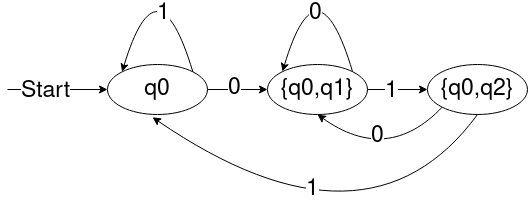
\includegraphics[scale = 0.5]{media/nfa_to_dfa.png}
		\centering
		\caption{Grafico DFA convertito da NFA}
	\end{figure}

	\newpage
	\subsection*{}
	\subsubsection*{Teorema}
	Se $D = (Q_N, \Sigma, \delta_N, q\textsubscript{0}, F_N)$ è il DFA trovato per costruzione a partire dal NFA $N = (Q_D, \Sigma, \delta_D, \{q_0\}, F_D)$ allora L(D)=L(N).

	\subsubsection*{Teorema}
	Un linguaggio L è accettato da un DFA se e solo se L è accettato da un NFA.

	\section{Automa con epsilon-transazioni}
	Un estensione degli automa è la capacità di poter ammettere come input la stringa vuota $\epsilon$. È come se l'NFA compisse una transizioni spontaneamente. Tale NFA si chiamerà $\epsilon$-NFA

	\subsection{Uso delle epsilon-transizioni}
	L'esempio di seguito tratta le $\epsilon$ come invisibili, possono mutare lo stato ma non sono contante nella catena.

	\begin{figure}[ht]
		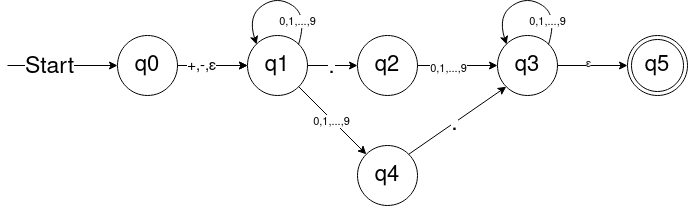
\includegraphics[scale = 0.5]{media/epsilon_nfa.png}
		\centering
		\caption{epsilon-NFA che accetta numeri decimali}
	\end{figure}

	L'$\epsilon$-NFA in figura accetta numeri decimali formati da:
	\begin{enumerate}
		\item un segno +,- facoltativo
		\item una sequenza di cifre
		\item un punto decimale
		\item una seconda sequenza di cifre
	\end{enumerate}
	È possibile avere input vuoti prima della virgola $\delta(q_1, .) = q_2$ e dopo la virgola $\delta(q_4, .) = q_3$ ma non entrambi. Il segno è facoltativo $\delta(q_0, \epsilon) = q_1$.
	\\ In $q_3$ l'automa può "scommettere" che la sequenza sia finita oppure può andare avanti a leggere.

	\newpage
	\subsection{Notazione formale di epsilon-NFA}
	La definizione forma di un $\epsilon$-NFA è uguale a quella di un NFA, va solo specificate le informazioni relative alla transizione $\epsilon$.
	\\ Una $\epsilon$-NFA è definita con $A = (Q, \Sigma, \delta, q_0, F)$, dove $\delta$ è una funzione di transizione che richiede come input:
	\begin{enumerate}
		\item uno stato \emph{Q}
		\item un elemento $\Sigma \cup \{\epsilon\}$, ovvero un simbolo di input oppure il simbolo $\epsilon$. Questa distinzione viene fatta per evitare confusione.
	\end{enumerate}

$\epsilon$-NFA per riconoscere un numero decimale
	\[ E = (\{q_0,q_1,...,q_5\}, \{.,+,-,1,...,9\},\delta, q_0, \{q_5\})\]

	\begin{table}[ht]
		\centering
		\begin{tabular}{c || c | c | c | c}
			      & $\epsilon$  & +,-         & .           & 0,1,...,9      \\
			\hline \hline
			$q_0$ & $\{q_1\}$   & $\{q_1\}$   & $\emptyset$ & $\emptyset$    \\
			$q_1$ & $\emptyset$ & $\emptyset$ & $\{q_2\}$   & $\{q_1, q_4\}$ \\
			$q_2$ & $\emptyset$ & $\emptyset$ & $\emptyset$ & $\{q_3\}$      \\
			$q_3$ & $\{q_5\}$   & $\emptyset$ & $\emptyset$ & $\{q_3\}$      \\
			$q_4$ & $\emptyset$ & $\emptyset$ & $\{q_3\}$   & $\emptyset$    \\
			$q_5$ & $\emptyset$ & $\emptyset$ & $\emptyset$ & $\emptyset$    \\
		\end{tabular}
		\caption{Tabella di transizione per un numero decimale}
	\end{table}

	\subsection{Epsilon chiusure}
	Un $\epsilon$-chiusura è un cammino fatto solo di transizioni $\epsilon$. Formalmente tale stato si scrive ENCLOSE(q) = {insieme di stati.}

	\subsection{Transizioni estese di epsilon-NFA}
	Grazie alle $\epsilon$-chiusure possiamo definire cosa significa accettare un input.
	\\
	Supponiamo $E = (Q, \Sigma, \delta, q_0, F)$ un $\sigma$-NFA, \circumdelta(q,w) è la funzione di transizione estesa le cui etichette concatenate descrivono la stringa w.
	\\
	\textbf{BASE} \circumdelta(q,w) = ENCLOSE(q), se l'etichetta è $\epsilon$ posso seguire solo cammini $\epsilon$, definizione di ENCLOSE.
	\\
	\textbf{INDUZIONE} Supponiamo \emph{w} abbia forma \emph{xa}, dove \emph{a} è l'ultimo simbolo, che non può essere $\epsilon$ perché non appartiene a $\Sigma$:
	\begin{enumerate}
		\item Poniamo \circumdelta(q,x) = $\{p_1, p_2,...,p_k\}$ in questo modo tutti i cammini $p_i$ sono tutti gli stati raggiungibili da q a x. Questi stati possono terminare con $\epsilon$ oppure contenere altre $\epsilon$ transizioni
		\item Sia $\bigcup^k_{i=1}\delta(p_i,a)$ l'insieme $\{r_1, r_2, ...,r_m\}$, ovvero tutte le transizioni da \emph{a} a \emph{x}.
		\item Infine \circumdelta(q,w) = $\bigcup^m_{j=1}ENCLOSE(r_j)$, questo chiude gli archi rimasti dopo \emph{a}
	\end{enumerate}
	Forma contratta
	\[\circumdelta(q,xa) = \bigcup_{p\in\circumdelta(q,x)}(\bigcup_{t\in\delta(q,a)}ENCLOSE(t))\]
	Il linguaggio accettato è L(E) = $\{w|\circumdelta(q_0,w) \cap F \ne 0\}$

	\subsection{Da epsilon-NFA a DFA}
	Dato un $\epsilon$-NFA possiamo costruire un equivalente DFA per sottoinsiemi. Sia $E = (Q_E, \Sigma, \delta_E, q_0, F_E)$ un $\epsilon$-NFA il suo equivalente DFA è
	\[ D = (Q_D, \Sigma, \delta_D, q_0, F_D) \]
	ovvero:
	\begin{enumerate}
		\item $Q_D$ è l'insieme di sottoinsiemi $Q_E$. Ogni stato accessibile in D è un sottoinsieme $\epsilon$-chiuso di $Q_E$, in termini formali S$\subseteq Q_E$ tale che S = ENCLOSE(S).
		\item $q_D$=ENCLOSE$(q_0)$
		\item $F_D$ contiene almeno uno stato accettante in E.
		      \\ $F_D=\{S|S$ è in $Q_D$ e $S \cap F_E\neq0\}$

		\item $\circumdelta(q,xa) = \bigcup_{p\in\circumdelta(q,x)}(\bigcup_{t\in\delta(q,a)}ENCLOSE(t))$
	\end{enumerate}
	\textbf{Teorema} Un linguaggio è linguaggio L è accetto da un $\epsilon$-NFA se è solo se è accettato da un DFA.

	\section{Espressioni regolari}
	Le espressioni regolari definiscono gli stessi linguaggi definiti dai vari automi: \emph{linguaggi regolari}. A differenza degli automi, le espressioni regolari descrivono linguaggi in maniera dichiarativa. Per questo motivo le espressioni regolari sono molto diffuse, per esempio nel commando unix \emph{grep} oppure negli analizzatori lessicali.

	\subsection{Operatori lessicali}
	L'espressione lessicale 01*+10* denota il linguaggio 0 seguito da qualsiasi numero di 1 oppure 1 seguito da qualsiasi numero di 0.
	\\ Per poter definire le operazioni sulle regex (sinonimo di espressione regolare) dobbiamo definire tali operazioni sui linguaggi che esse rappresentano:
	\begin{enumerate}
		\item \emph{Unione} di due linguaggi L ed M, L$\cup$M, indica tutte le stringhe che appartengono ad L e ad M oppure a entrambi.
		\item \emph{Concatenazione} di due linguaggi L ed M è l'insieme di stringhe formate dalla concatenazione di una qualsiasi stringa L con una qualsiasi stringa M. Tale operazione è indicata così: L$\cdot M$ oppure semplicemente LM.
		      Per L=\{001,10,111\} e M=\{$\epsilon$,001\}
		      LM=\{001,10,111,001001, 10001, 111001\}
		\item \emph{Chiusura}(o \emph{star} o chiusura di Kleene) di un linguaggio L, indicata come L*, rappresenta l'insieme delle stringhe che si possono formare tramite concatenazione e ripetizione di qualsiasi stringa in L. Nel caso L=\{0,1\} L* rappresenta l'alfabeto binario, qualsiasi combo di 0 e 1. Nel caso L=\{0, 11\} L* rappresenta qualsiasi stringa che abbia una o più coppie di 1, NB 011 è valido ma come 01111, mentre 101 non è valido, non abbiamo né la stringa 10 né la stringa 01. Formalmente L* è l'unione infinita $\bigcup_{i>0}L_i$ dove $L^0=\{\epsilon\}$, $L^1=L$, $L^i=LL...L$.
	\end{enumerate}

	\newpage
	\subsection{Proprietà regex}
	\begin{outline}
		\1 $L\cup M=M\cup L$ L'unione è commutativa
		\1 $(L\cup M) \cup M= L\cup (M\cup L)$ L'unione è associativa
		\1 $(LM) M= L (M L)$ La concatenazione è associativa (LM $\neq$ ML)
		\1 $\emptyset \cup L= L \cup \emptyset=L$
		\1 $\{\epsilon\} \cup L= L \cup \{\epsilon\}=L$
		\1 $\emptyset L= L \emptyset=\emptyset$
		\1 $L(M\cup N)= LM \cup LN$
		\1 $(M\cup N)L=ML\cup NL$
		\1 $L\cup L=L$
		\1 $\emptyset^*=\{\epsilon\}, \{\epsilon\}^* =\{\epsilon\}$
		\1 $L^+=LL^*=L^*L,\;L^*=L^*\cup \{\epsilon\}$
	\end{outline}

	\newpage
	\subsection{Costruzione di regex}
	Servono modi per raggruppare le espressioni regolari, in questo caso vengono usati operatori algebrici comuni. Di seguito verranno definite regex lecite E con il loro corrispondente linguaggio L(E).
	\\ \textbf{BASE}
	\begin{enumerate}
		\item le costanti $\epsilon$ e $\emptyset$ sono regex, rispettivamente del linguaggio \{$\epsilon$\} e \{$\emptyset$\}, in altri termini L($\epsilon$) =\{ $\epsilon$\} e L($\emptyset$) = \{$\emptyset$\}.
		\item Se a è un simbolo allora \textbf{a} è una regex che denota il linguaggio \{a\}, ovvero L(\textbf{a}) = \{a\}. (si usa il grassetto per distinguere simboli da regex)
		\item Una lettera maiuscola qualsiasi, di solito \emph{L}, viene usata per indicare un linguaggio arbitrario
	\end{enumerate}
	\textbf{INDUZIONE}
	\begin{enumerate}
		\item Data \emph{E} ed \emph{L} regex, allora \emph{E} + \emph{L} è una regex che indica l'unione dei due linguaggi L(\emph{E}) e L(\emph{L}), in altre parole L(\emph{E+F}) = L(\emph{E}) $\cup$ L(\emph{F})
		\item Date \emph{E} e \emph{F} due regex, \emph{EF} indica la concatenazione tra i due linguaggio L(\emph{E}) e L(\emph{F}), in altri termini L(\emph{EF}) = L(E)L(F).
		\item Data \emph{E} una regex, \emph{E}* indica la chiusura del linguaggio L(\emph{E}), in altri termini L(\emph{E}*) = (L(\emph{E}))*
		\item Data \emph{E} una regex, allora anche (\emph{E}) è una regex valida che appartiene sempre al linguaggio \emph{E}, in termini formali L((\emph{E})) = L(\emph{E})
	\end{enumerate}
	\textbf{Esempio di regex}
	\\ Si crei una regex che descriva una linguaggio che è fatto di 0 e 1 alternati.
	\\ Intuitivamente si potrebbe provare \textbf{01}*, che è errato, questo indica tutte le stringhe che hanno uno 0 e un numero arbitrario di 1. (\textbf{01})* è corretto, però indica per forza un linguaggio di 01 alternati, quindi 101010 non sarebbe valido
	\\ Uniamo regex per descrivere il caso: (\textbf{10}*) 10 alternato,
	\textbf{0(10)*} 10 con 0 all'inizio,
	\textbf{1(01)*} 01 con 1 all'inizio,
	in conclusione
	\[\textbf{(01)*+(10)*+0(10)*+1(01)*}\]
	Un modo più contratto sarebbe quello di aggiungere un 1 facoltativo all'inizio e uno 0 facoltativo alla fine
	\[\textbf{($\epsilon$+1)(01)*)($\epsilon$+0)}\]

	\subsection{Precedenza degli operatori}
	\begin{enumerate}
		\item Star ha la precedenza massima
		\item concatenazione
		\item unione
	\end{enumerate}
	Naturalmente si possono usare parentesi per decidere il proprio ordine e inoltre è consigliato farlo anche se non fosse necessario per rendere più chiara l'espressione.

	\section{Automa a stati finite e regex}
	Abbiamo visto che le regex e gli automi a stati finiti possono descrive gli stessi linguaggi, va solo dimostrato che formalmente.
	\\ Dobbiamo dimostrare che:
	\begin{enumerate}
		\item Ogni linguaggio definito da un automa è definito anche da una regex, useremo un DFA per comodità
		\item Ogni linguaggio definito da una regex è definita da un automa, useremo un $\epsilon$-NFA per comodità
	\end{enumerate}

	\begin{figure}[ht]
		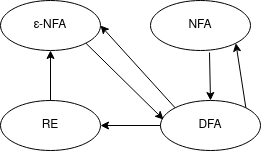
\includegraphics[scale = 0.7]{media/regex_conv.png}
		\centering
		\caption{Conversioni}
	\end{figure}

	\subsection{Da DFA a regex}
	\textbf{Teorema}
	\\ Se L = L(A) per un DFA A, allora esiste una regex \emph{R} tale che L = L(\emph{R}).
	\\ Il procedimento formale e matematico è formato dal espansione di ogni singolo stato tramite la formula:
	\[ R^{k}_{ij} =  R^{k-1}_{ij} + R^{k-1}_{ik} (R^{k-1}_{kk} R^{k-1}_{kj})\]
	In parole povere sto calcolando l'espressione regolare da uno stato j a uno stato i k volte, una per ogni stato.
	\\ Questo procedimento è molto lungo, perché l'espressione va effettuata per ogni transizione, unita e poi ridotta.
	\\ Tenendo però a mente questa formalità è possibile usare un metodo più gestibile, ovvero \emph{l'eliminazione per stati}.

	\newpage

	\begin{figure}[ht]
		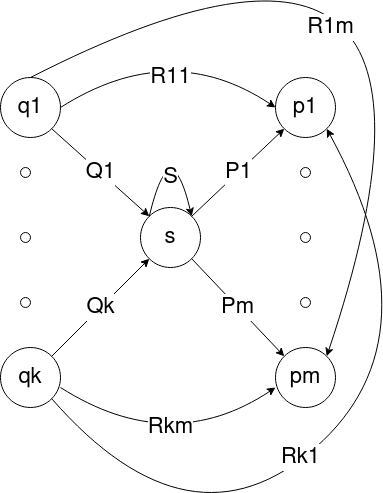
\includegraphics[scale = 0.5]{media/regex_dfa.png}
		\centering
		\caption{Eliminazione per stati}
	\end{figure}

	\begin{outline}
		\1 \emph{s} è lo stato generico che sta per essere eliminato
		\1 $q_1, q_2,...,q_k$ sono i k stati precedenti a \emph{s}
		\1 $Q_i$ sono tutte le transizioni precedenti
		\1 $p_1, p_2,...,p_k$ sono i k stati successi a \emph{s}
		\1 $P_i$ sono tutte le transizioni successive
		\1 $R_{ij}$ sono tutte le transizioni tramite regex, bisogna definirne una per ogni direzione \emph{ij} ma se non dovesse esistere basterà scrivere $\emptyset$
	\end{outline}

	\begin{figure}[ht]
		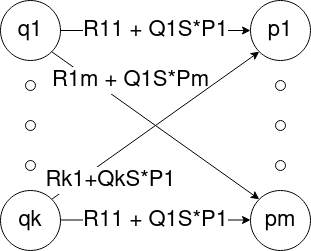
\includegraphics[scale = 0.5]{media/removed_s.png}
		\centering
		\caption{Eliminazione di s}
	\end{figure}

	A questo punto possiamo iniziare a costruire l'espressione regolare a partire dall'automa.
	\newpage
	\begin{enumerate}
		\item Bisogna eliminare tutti gli stati intermedi ad eccezione di $q_0$.
		\item Se $q_0\neq q_1$ allora questo stato può essere espresso come $E_q$ = (R + SU*T)*SU*, un cammino generico illustrato in figura.

		      \begin{figure}[ht]
			      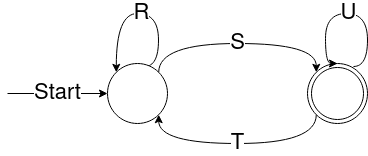
\includegraphics[scale = 0.5]{media/automa_generico.png}
			      \centering
			      \caption{Automa generico 2 stati}
		      \end{figure}

		\item Se $q_0$ è accettante allora la regex è data da R*

		      \begin{figure}[ht]
			      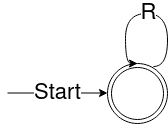
\includegraphics[scale = 0.5]{media/automa_q0.png}
			      \centering
			      \caption{Automa generico 1 stato}
		      \end{figure}

	\end{enumerate}

	\newpage
	Dato un NFA come segue.

	\begin{figure}[ht]
		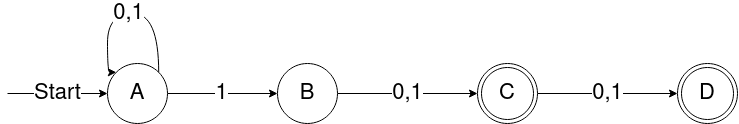
\includegraphics[scale = 0.5]{media/dfa_s1.png}
		\centering
		\caption{NFA esempio}
	\end{figure}

	Esprimiamo le sue funzioni di transizioni come regex

	\begin{figure}[ht]
		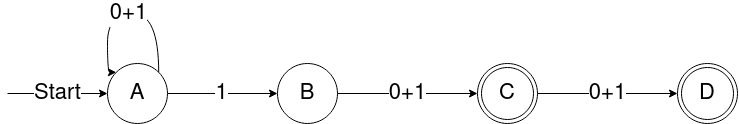
\includegraphics[scale = 0.5]{media/dfa_s2.png}
		\centering
		\caption{NFA con archi regex}
	\end{figure}

	Il primo stato che rimuoviamo è B, applicando la fromula. $R_{11} + Q_1 S^* P_1$, in questo caso risulta $\emptyset + 1\emptyset$*(0+1), che si può  ridurre in 1(0+1).
	\\ NB $\emptyset$* equivale a $\epsilon$, non annulla le regex, mentre $\emptyset$ sì


	\begin{figure}[ht]
		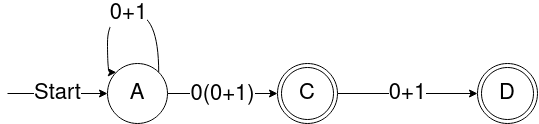
\includegraphics[scale = 0.5]{media/dfa_s3.png}
		\centering
		\caption{B rimosso}
		\label{b rimosso}
	\end{figure}

	\newpage
	Eliminiamo C

	\begin{figure}[ht]
		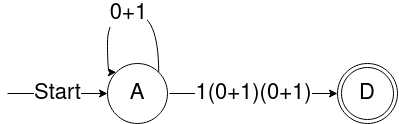
\includegraphics[scale = 0.5]{media/dfa_s4.png}
		\centering
		\caption{C rimosso}
	\end{figure}

	Ora possiamo applicare (R + SU*T)*SU*, quindi
	\begin{itemize}
		\item R=(0+1)
		\item S=1(0+1)(0+1)
		\item T=$\emptyset$
		\item U=$\emptyset$.
	\end{itemize}
	\[((0+1) + 1(0+1)(0+1)\emptyset^*\emptyset)^*1(0+1)(0+1)\emptyset\]
	Possiamo semplificare U* perché è equivalente a $\epsilon$ e possiamo eliminare SU*T perché è T è $\emptyset$.
	\[(0+1)^*1(0+1)(0+1)\]
	Questo è lo stato accettante D, è necessario calcolare lo stato accettante C. Ripartendo dalla fig.\ref{b rimosso} applichiamo di nuovo $E_Q$ ottenendo (0+1)*1(0+1).
	\\ L'espressione finale è data dalla \textbf{somma} delle 2 espressioni.
	\[(0+1)*1(0+1) + (0+1)^*1(0+1)(0+1)\]

	\newpage
	\subsection{Da regex a automi}
	\textbf{Teorema} Per ogni rex R possiamo costruire un $\epsilon$-NFA A tale che L(R)=L(A).
	\\ Questo si dimostra per induzione strutturale, prendendo come base gli automi $\epsilon$, $\emptyset$ e \emph{a}.

	\begin{figure}[ht]
		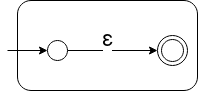
\includegraphics[scale = 0.5]{media/epsilon.png}
		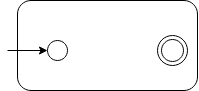
\includegraphics[scale = 0.5]{media/empty.png}
		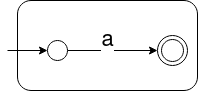
\includegraphics[scale = 0.5]{media/simple_a.png}
		\centering
		\caption{Stati base}
	\end{figure}


	\begin{figure}[ht]
		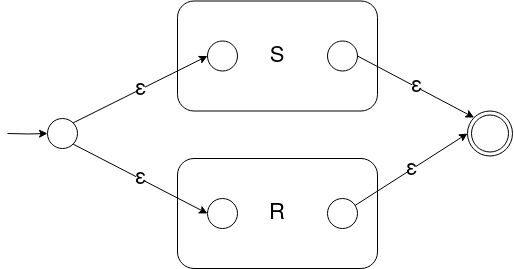
\includegraphics[scale = 0.4]{media/RS.png} \\ \\
		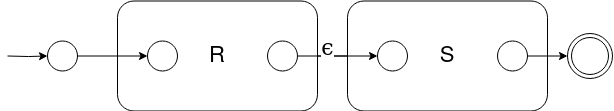
\includegraphics[scale = 0.4]{media/RSmult.png} \\ \\
		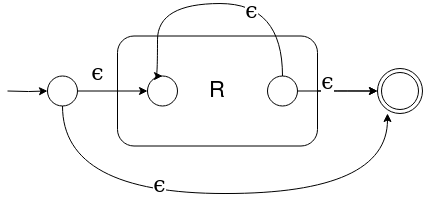
\includegraphics[scale = 0.4]{media/RSstar.png}
		\centering
		\caption{R+S, RS e R*}
	\end{figure}

	R+S significa che viene percorso 1 dei 2 espressioni. RS significa che una volta percorso R, quello diventa lo stato iniziale di S. R* va in loop su se stesso.

	\newpage
	Usando i blocchi precedenti convertiamo (0+1)*1(0+1)

	\begin{figure}[ht]
		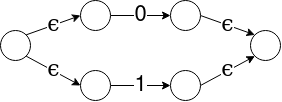
\includegraphics[scale = 0.4]{media/01.png} \\ \\
		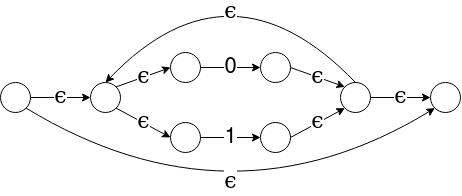
\includegraphics[scale = 0.4]{media/01star.png} \\ \\
		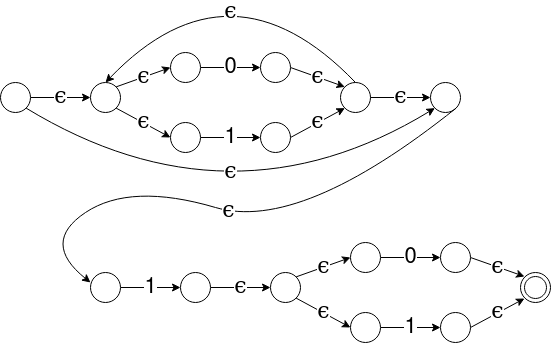
\includegraphics[scale = 0.4]{media/01star01.png}
		\centering
		\caption{R+S, RS e R*}
	\end{figure}

	\section{Proprietà dei linguaggi regolari}
	\begin{outline}
		\1 \emph{Pumping Lemma}: Ogni linguaggio regolare soddisfa il pumping di lemma
		\1 \emph{Proprietà di chiusura}: Possibilità di costruire un nuovo automa a partire da altri automi, seguendo specifiche operazioni
		\1 \emph{Proprietà di decisione}: Analisi di automi, come l'equivalenza
		\1 \emph{Tecniche di minimizzazione}: Possiamo ridurre un automa
	\end{outline}

	\subsection{Pumping Lemma}
	Un linguaggio non è detto che sia regolare.
	\\ Immaginiamo di avere un linguaggio $L_{01}=\{0^n\;1^n|n\geq 1\}$. Questo è un linguaggio che accetta una stringa con tanti 1 quanti 0. Perché questo linguaggio possa essere un DFA deve avere un numero finito di stati, diciamo $k$. Quindi dopo $k+1$ simboli, $\epsilon,0,00,...,0^k$ ci troviamo in un qualche stato. Poiché gli stati sono limitati esistono 2 strade diverse per cui ci troviamo nello stesso stato, chiamiamoli $0^j$ e $0^i$.
	\\ Ora immaginiamo dallo stato $j$ di iniziare a leggere 1, l'automa deve fermarsi quando ha letto $j$ quantità di 1, ma non può farlo perché non ricorda lo stato, potrebbe finire dopo $i$ quantità di 1, $L_{01}$ non è regolare.
	\\ \textbf{Teorema} Sia L un linguaggio regolare, allora esiste una costante $n$ tale che, per ogni stringa $w$ in $L$ dove $|w|\geq n$ possiamo scomporre $w$ in 3 stringhe $w=xyz$ tale che:
	\begin{enumerate}
		\item $y \neq \epsilon$
		\item $|x,y| \leq n$
		\item per ogni $k \geq 0$ anche $xy^kz$ è in $L$
	\end{enumerate}
	Ovvero c'è una stringa non vuota replicabile da qualche parte, senza uscire dal linguaggio.
	\\ \textbf{Dimostrazione} Supponiamo che $L$ sia regolare. Allora L=L(A) e supponiamo che $A$ abbia $n$ stati. Ora consideriamo una stringa $w$ dove $w=a_1,a_2,...,a_m \; m \geq n$ e ogni $a_i$ è un simbolo di input. Definiamo la sua funzione $\delta(a_1,a_2,...,a_n)$ che descrivere tutte le $p_i$ transizioni, e $q_0=p_0$.
	\\ Per il principio della piccionata tutti gli stati non possono essere distinti, quindi esistono due stati $p_i$ e $p_j$ dove $0 \leq i \leq j \leq n$ tale che $p_i = p_j$. Possiamo scomporre w in w=xyz:

	\begin{enumerate}
		\item $x=a_1,a_2,...,a_i$
		\item $y=a_{i+1},a_{i+2},...,a_j$
		\item $x=a_{j+1},a_{j+2},...,a_m$
	\end{enumerate}

	\begin{figure}[ht]
		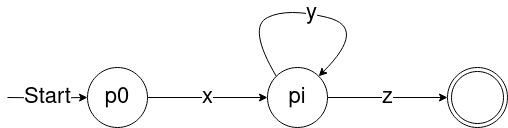
\includegraphics[scale = 0.5]{media/pump.png}
		\centering
		\caption{A un certo punto i stati si ripetono}
	\end{figure}

	Se k=0 siamo allo stato accettante, se $k \geq 0$ allora dobbiamo necessariamente fare dei loop, perché l'input è $xy^kz$.

	\newpage
	\subsection{Chiusura dei linguaggi regolari}
	Sia $L$ e $M$ due linguaggi regolari allora i seguenti sono a loro volta linguaggi regolari.
	\begin{outline}
		\1 \emph{Unione}: $L \cup M$
		\1 \emph{Intersezione}: $L \cap M$
		\1 \emph{Complemento}: $N$
		\1 \emph{Differenza}: $L \backslash M$
		\1 \emph{Inversione}: $LR = \{wR : w \in L\}$
		\1 \emph{Chiusura}: $L^*$
		\1 \emph{Concatenazione}: $L\cdot M$
	\end{outline}

	\textbf{Teorema} Sia L e M linguaggi regolari allora anche L $\cup$ M è un linguaggio regolare.
	\\ \textbf{Dimostrazione} L ed M sono linguaggi descritti dalle espressioni regolari S ed R, quindi L=L(S) e M=L(R) quindi L$\cup$M=L(R+S).
  \vspace{5mm}

\textbf{Teorema} Se L è un linguaggio regolare sull'alfabeto $\Sigma$ allora anche $\overline{L}=\Sigma^*-L$.
\\ \textbf{Dimostrazione} Sia L=L(A) per un DFA A=$(Q,\Sigma,\delta,q_0,F)$, allora $\overline{L}$=L(B) dove B è il DFA $(Q,\Sigma,\delta,q_0,Q-F)$, quindi B ha gli stati accentanti opposti a quelli di A. In questo caso l'unico modo per cui $w$ è in L(B) se e solo se $\delta(q_0,w)$ è in $Q-F$, ovvero \textbf{non} è in L(A).

\begin{figure}[ht]
  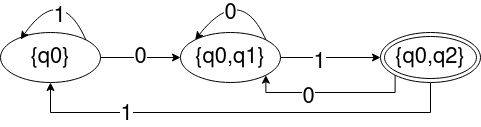
\includegraphics[scale = 0.5]{media/prop1.png}
  \centering
  \caption{Diagramma di A}
\end{figure}

\newpage
Il diagramma di B risulta opposto
\begin{figure}[ht]
  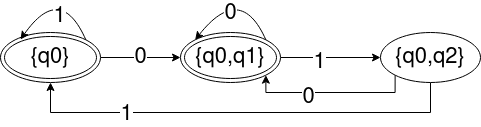
\includegraphics[scale = 0.5]{media/prop2.png}
  \centering
  \caption{Diagramma di B}
\end{figure}

\textbf{Teorema} 4.8. Se $L$ e $M$ sono regolari, allora anche $L \cap M$ è regolare.
\vspace{5mm}
\\ \textbf{Dimostrazione} Le 3 operazioni booleane sono interdipendenti, quindi possiamo usare le due precedenti per dimostrare l'Intersezione
\[L\cap M = \overline{\overline{L} \cup \overline{M}}\]
\\ \textbf{Dimostrazione alternativa} Sia L il linguaggio $L = (Q_L, \Sigma, \delta_L, q\textsubscript{0}, F_L)$ e M il linguaggio
$M = (Q_M, \Sigma, \delta_M, q\textsubscript{0}, F_M)$ assumiamo per semplicità che siano dei DFA
Se $A_L$ passa da $p$ a $s$ e $A_M$ passa da $q$ a $t$ (sono tutti stati) allora $A_{L\cap M}$ passera da $(p,s) a (q,t)$ quando legge una stringa $a$.
\\ Formalmente il linguaggio risultante dall'intersezione diventa 
\[A = (Q_M \times Q_L, \Sigma, \delta_{M\cap L}, (q_M, q_L), F_L \times F_M)\]
Si può dimostrare che $\circumdelta((q_M,q_L),w) = (\circumdelta(q_M, w), \circumdelta(q_L,w))$, questo perché A accetta solo quando entrambi gli stati sono accettanti, quindi accetta per forza anche l'intersezione. 

\subsubsection{Chiusura rispetto alla differenza} 
\textbf{Teorema} Sia $L$ e $M$ dei linguaggi regolari allora anche $L-M$ è un linguaggio regolare
\vspace{5mm}
\\ \textbf{Dimostrazione} $L-M=L\cap \overline{M}$, ma sappiamo che $\overline{M}$ è regolare e l'intersezione di 2 linguaggi è regolae, quindi $L-M$ è anche esso regolare.

\subsubsection{Inversione}
L'inversione di una strina $a_1, a_2, ...,a_n$ è la stringa $a_n,..., a_2, a_1$ questa stringa la denotiamo come $w^R$ e notiamo che $\epsilon^R=\epsilon$.
\\ Un linguaggio $L^R$ inverso di $L$ presenta tutte le stringe al suo interno inverse. Se $L$ è un linguaggio regolare allora lo è anche $L^R$.

\subsection{Proprietà di decisione}
Questi non scontanti che vanno affrontate:
\begin{itemize}
  \item Un linguaggio descritto è vuoto?
  \item Una stringa appartiene al linguaggio?
  \item Due linguaggi equivalenti?
\end{itemize}

\subsubsection{Verificare se un linguaggio è vuoto}
Se il linguaggio $A$ è rappresentato da un automa finito posso attraversare tutti i nodi, se trovo uno stato accettante allora il linguaggio \textbf{non} è vuoto. Quest'operazione richiede O($n^2$) perché è un semplice attraversamento di grafo. 
\\ Se iniziamo da un espressione regolare, possiamo trasformarla in un $\epsilon$-NFA e poi effettuare i cammini a costo O(n).
\\ È possibile anche determinare se il linguaggio è vuoto in base alla regex direttamente. Se il linguaggio non ha $\emptyset$ sicuramente non può essere vuoto, altrimenti posso determinarlo ricorsivamente seguendo le regole algebriche delle regex. 
\\ Di seguito elenco i casi: 
\begin{itemize}
  \item $R= \emptyset$. $L(\emptyset)$ è vuoto
  \item $R= \epsilon$. $L(\epsilon)$ \textbf{non} è vuoto
  \item $R=a$ (qualsiasi stringa $a$) L(a) non è vuoto
  \item $R=R_1+R_2$. $L(R)$ è vuoto se sia $L(R_1)$ che $L(R_2)$ siano vuoti
  \item $R=R_1R_2$. $L(R)$ è vuoto se $L(R_1)$ o $L(R_2)$ è vuoto
  \item $R=R_1*$. $L(R)$ non è mai vuoto, al massimo è $\epsilon$
  \item $R=R_1$. $L(R)$ è vuoto solo se $L(R_1)$ è vuoto, sono lo stesso linguaggio
\end{itemize}

\subsubsection{Appartenenza a un linguaggio}
Per controllare se una qualsiasi stringa $w\in L(A)$ per un DFA è sufficiente simulare w su A, se $|w|=n$ il tempo risulta O(n).
\vspace{5mm} \\
Se $A$ è un NFA e ha $s$ stati, allora O($ns^2$), vale lo stesso epr $\epsilon$-NFA.
\vspace{5mm} \\
Se L=L(R) è una regex, la converto in $\epsilon$-NFA ovvero O($ns^2$)

\subsubsection{Equivalenza e minimizzazione di automi}
Dobbiamo esplorare la possibilità di dire che 2 DFA sono equivalenti, un modo per farlo è minimizzarli, se sono equivalenti basterà cambiare etichette finché non coincidono.
\\ Iniziamo definendo cosa rende equivalenti 2 stati $p$ e $q$. Data una stringa $w$, $p$ e $q$ sono equivalenti se \circumdelta$(q,w)$ e \circumdelta$(p,w)$ sono entrambi accentanti oppure non accentanti. 
\\ Nel caso in cui uno sia accentante e l'altro no, allora si dicono distinti. NB. 2 stati equivalenti non ci dicono niente sulla stringa $w$ e non ci dice se i due stati sono lo stesso. 
\\ Possiamo raggruppare le nostre distinzioni degli stati in una tabella, tramite l'algoritmo $riempit-tabella$.

\begin{figure}[ht]
	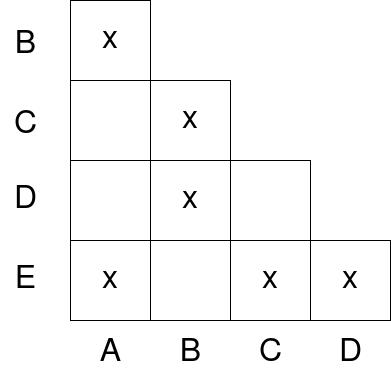
\includegraphics[scale = 0.3]{media/riemp_tab.png}
	\centering
	\caption{Algoritmo riempi tabella}
\end{figure}
Ogni x è uno stato distinguibile, un quadrato vuoto significo stati equivalenti.
\\ Per testare se 2 linguaggi L e M sono equivalenti dobbiamo: 
\begin{itemize}
  \item Convertire L e M in DFA 
  \item Costruire il DFA unione dei 2 linguaggi
  \item Se l'algoritmo dice che i 2 stati iniziali sono equivalenti allora L=M, altrimenti L$\ne$M
\end{itemize}

Partendo da 2 DFA costruisco un DFA $B$ che ha lo stato iniziale che contiene quello di $A$ e lo stato accentante che contiene quello di $A$. Ogni altra funzione di un blocco deve essere equivalente.
\\ L'algoritmo non può essere applicato a un NFA.

\section{Grammatiche libere da contesto}
\textbf{Esempio informale}
\vspace{5mm}
\\ Definiamo un linguaggio delle palindrome. Una stringa è palindroma se si legge allo stesso modo in entrambi i versi, come $otto$ oppure $madamimadam$ (madame I'm Adam). Perciò $w$ è palindroma se $w=w^R$. 
\\ Si può facilmente dimostrare che questo linguaggio non è regolare usando il pumping lemma. Scegliamo $w=0^n10^n$, scomponiamo in $w=xyz$ tale che y sia fatto di vari 0 e scegliamo k=0, $xz$ dovrebbe adesso appartenere a $L_{pal}$ ma non è così, perché ho meno 0 a sinistra rispetto che a destra. 
\\ Posso definire le stringhe che appartengono a $L_{pal}$ in maniera ricorsiva. 
\vspace{2mm}
\\ \textbf{Base} $\epsilon$, 0 e 1 sono palindrome
\\ \textbf{Induzione} Se $w$ è palindroma allora $0w0$ e $1w1$ sono palindrome
\vspace{2mm}
\\ Una \textbf{grammatica libera} è una notazione formale per esprimere linguaggi ricorsivamente. Una grammatica consiste in una o più serie di variabili che rappresentano classi di stringhe, ovvero linguaggi.
\\ Ogni classe definisce come costruire le stringhe in ogni classe. Definiamo le classi del linguaggio palindroma:
\begin{enumerate}
  \item $P\rightarrow\epsilon$
  \item $P\rightarrow0$
  \item $P\rightarrow1$
  \item $P\rightarrow 0P0$
  \item $P\rightarrow 1P1$
\end{enumerate}
0 e 1 sono terminali, P è una variabile, P è anche la categoria iniziale, 1-5 sono produzioni.

\newpage
\subsection{Definzione formale di CFG}
Un CFG è formato da 4 elementi: 
\begin{enumerate}
  \item Un insieme di simboli detti \emph{terminali}
  \item Un insieme di variabili, detti \emph{non termali} oppure \emph{categorie sintattiche}
  \item Una variabile detto \emph{simbolo iniziale}
  \item Un insieme finito di \emph{produzioni} o \emph{regole} che definiscono il linguaggio ricorsivamente. Ogni produzione consiste in 3 parti 
    \begin{enumerate}
      \item Una variabile che è definita parzialmente dalla produzione, \emph{testa}
      \item Il simbolo di produzione $\rightarrow$
      \item Il \emph{corpo} della produzione, ovvero la stringa o il terminale che la forma. Le stringhe vengono formate sostituendo le variabili.
    \end{enumerate}
\end{enumerate}
In maniera contratta, CFG=(V,T,P,S) rispettivamente variabile, terminale, produzioni e simbolo iniziale. 
\\ Il linguaggio palindromo descritto come CFG è $G_{pal}=(\{P\}, \{0,1\},A,P)$ A è l'insieme delle produzioni del linguaggio.

\subsection{Derivazione in CFG}
Possiamo definire le stringhe tramite concatenazione delle produzione, \emph{inferenza ricorsiva} 
\\ Il secondo modo per \emph{derivazione}, ovvero uso le produzioni fino a quanto ho solo simboli terminali. Noi studieremo la derivazione.
\\ Sia $G=(V,T,P,S)$ una grammatica libera e sia $\alpha AB$ una stringa mista di terminali e variabili, dove $A$ è variabile e $\alpha B \in (V \cup T)$ allora se $G$ risulta chiara nel contesto, posso scrivere: 
\[\alpha A B \xRightarrow[G] \; \alpha \gamma B\]
$A$ è una derivazione di $G$, $A \Rightarrow \gamma $. Posso usare il simbolo * per denotare "zero o più passi"(chiusura transitiva). 
\\ \textbf{Base} $\alpha \xRightarrow[G]{*} \alpha$, vale per ogni stringa terminale o variabile, ovvero ogni stringa deriva se stessa 
\\ \textbf{Induzione} Se $\alpha \xRightarrow[G]{*} \beta$ e $\beta \xRightarrow[G]{} \gamma$ significa che $\alpha \xRightarrow[G]{*} \gamma$
\\ Se la grammatica è chiara posso scrivere $\xRightarrow{*}$

\subsection{Derivazione a sinistra e a destra}
È possibile arrivare a diverse conclusioni a seconda della scelta di quali produzioni fare, quindi per evitare di avere incertezze si può scegliere un verso di come derivare ogni volta.
\\ Derivazione a destra: $\xRightarrow[rm]{}$
\\ Derivazione a sinistra: $\xRightarrow[lm]{}$

\subsection{Linguaggio di una grammatica}
Se $G(V,T,P,S)$ è una CFG allora il suo linguaggio è:
\[L(G)=\{ w \in T^*:S \xRightarrow[G]{*} w \}\]
Ovvero l'insieme delle stringhe $T^*$ derivabili da $w$

\subsection{Alberi sintattici}
Data una grammatica $G=(V,T,S,P)$, gli alberi sintattici di $G$ soddisfano i seguenti requisiti: 
\begin{enumerate}
  \item Ogni nodo interno è una variabile $V$
  \item Ogni foglia è un variabili, terminale o $\epsilon$. Quando è $\epsilon$ deve essere l'unico figlio
  \item Se un nodo $A$ con i figli $X_1,X_2,...,X_k$ allora $A \rightarrow X_1,X_2,...,X_k$ è una produzione in $P$. $X$ può essere $\epsilon$ solo nel caso in qui $A \rightarrow \epsilon$
\end{enumerate}

Nella grammatica seguente: 
\begin{enumerate}
  \item $E \rightarrow I$
  \item $E \rightarrow E+E$
  \item $E \rightarrow E*E$
  \item $E \rightarrow (E)$
\end{enumerate}

\begin{figure}[ht]
  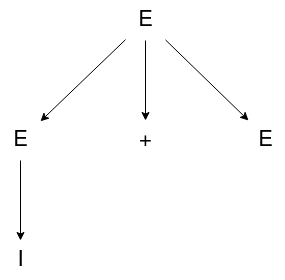
\includegraphics[scale = 0.5]{media/produzione.png}
  \centering
  \caption{Parsing tree}
\end{figure}
\newpage
Questo albero sintattico rappresenta la produzione 
$E \xRightarrow[]{*} I + E$

\subsubsection{Prodotto di un albero sintattico} 
Se concateniamo le foglie di un albero otteniamo una stringa, ovvero il \emph{prodotto}. Inoltre la radice deve essere il simbolo iniziale e ogni foglia è $\emptyset$ oppure un terminale. 

\begin{figure}[ht]
	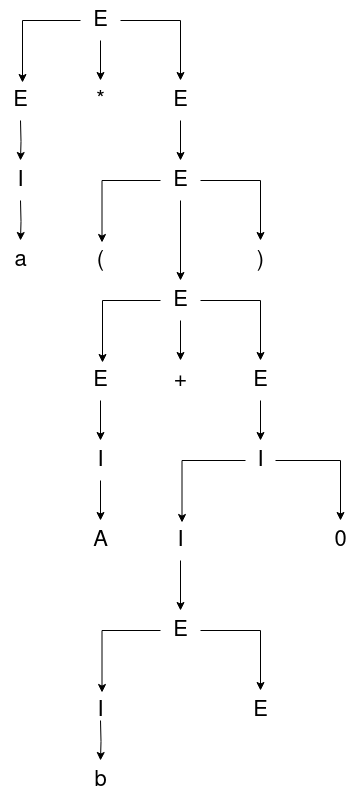
\includegraphics[scale = 0.3]{media/prod_concat.png}
	\centering
	\caption{Produzione}
  \label{prod}
\end{figure}
\newpage
Il risultato della produzione è $a*(a+b00)$

\subsubsection{Inferenza, derivazione e alberi sintattici}
Sia $G=(V,T,P,S)$ una CFG e $A \in V$ allora i seguenti sono equivalenti: 
\begin{enumerate}
  \item $A \xRightarrow[]{*} w$ 
  \item $A \xRightarrow[lm]{*} w$ 
  \item $A \xRightarrow[rm]{*} w$ 
  \item C'è un albero sintattico $G$ con radice $A$ e prodotto $w$
\end{enumerate}
Costruiamo il prodotto della fig. \ref{prod} per derivazione sinistra: 
\begin{itemize}
  \item $ E \xRightarrow[lm]{} E * E \xRightarrow[lm]{}$
  \item $ I * E \xRightarrow[lm]{} $
  \item $ a * E \xRightarrow[lm]{} $
  \item $ a * (E) \xRightarrow[lm]{} $
  \item $ a * (E+E) \xRightarrow[lm]{} $
  \item $ a * (I+E) \xRightarrow[lm]{} $
  \item $ a * (a+E) \xRightarrow[lm]{} $
  \item $ a * (a+I) \xRightarrow[lm]{} $
  \item $ a * (a+I0) \xRightarrow[lm]{} $
  \item $ a * (a+I00) \xRightarrow[lm]{} $
  \item $ a * (a+b00) \xRightarrow[lm]{} $
\end{itemize}

\subsection{Ambiguità in grammatiche e linguaggi}
Nella grammatica: 
\begin{itemize}
  \item $E \rightarrow I$ 
  \item $E \rightarrow E+E$ 
  \item $E \rightarrow E*E$ 
  \item $E \rightarrow (E)$ 
\end{itemize}
L'espressione $E+E*E$ ha due possibili derivazioni: 
$E \Rightarrow E + E \Rightarrow E + E * E$ oppure 
$E \Rightarrow E * E \Rightarrow E + E * E$, da qui i due alberi sintattici

\begin{figure}[ht]
  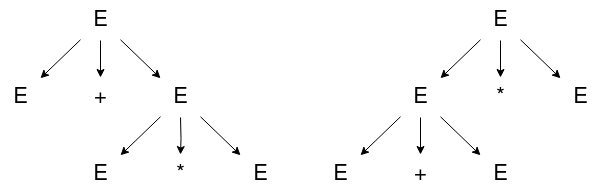
\includegraphics[scale = 0.5]{media/ambigua.png}
  \centering
  \caption{Semplice automa}
\end{figure}

\newpage 
Queste sono 2 operazioni diverse, usiamo i valori $1+2*3$, dal primo albero troviamo $1+(2*3)=7$ mentre dal secondo albero troviamo $(1+2)*3=9$.
\\ \textbf{Definizione} Sia $G=(V,T,P,S)$ una CFG. Diciamo che G è ambigua se esiste almeno una stringa T* che ha più di un albero sintattico. 

\subsubsection{Rimuovere ambiguità}
È possibile, in alcuni casi, rimuovere l'ambiguità. Non esiste però un modo sistematico e alcuni CFL hanno solo CFG ambigue. 
\\ Studiamo la grammatica 
\[ E \rightarrow I \;|\; E + E \;|\; E * E \;|\; (E)\]
\[ I \rightarrow a \;|\; b \;|\; Ia \;|\; Ib \;|\; I0 \; | \; I1\]
Dobbiamo decidere: 
\begin{enumerate}
  \item Chi ha precedenza tra + e *
  \item Come raggruppare un operatore
\end{enumerate}
Una soluzione è l'introduzione di una gerarchia di variabili: 
\begin{enumerate}
  \item espressioni E: composizione di uno o più termini T tramite +
  \item termini T: composizione di uno o più fattori F tramite *
  \item fattori F:
    \begin{enumerate}
      \item identificatori I
      \item espressioni E racchiuse tra parentesi
    \end{enumerate}
\end{enumerate}
Ogni più è costretto a essere una T, ogni T può generare E solo chiuse nelle parentesi, questo significa che * ha precedenza rispetto al +. 
\\ La seguente grammatica risulta quindi non ambigua: 
\begin{enumerate}
  \item $E \rightarrow T | E + T$
  \item $E \rightarrow F | T * F$
  \item $F \rightarrow I | (E) $
  \item $E \rightarrow a | b | Ia | Ib | I0 | I1$
\end{enumerate}

\subsubsection{Ambiguità inerente} 
Un CFL è inerentemente ambiguo se tutte le grammatiche per L sono ambigue. 
\[ L = \{a^n b^n c^m d^m :n \geq 1, m \geq 1\} \cup \{a^n b^m c^m d^n : n \geq 1, m \geq 1\} \]
Il linguaggio è inerentemente ambiguo.

\section{Automi a pila}
Un automa a pila (PDA - pushdown automaton) è un $\epsilon$-NFA con una pila che è la sua memoria.
\\ Durante le transizione:
\begin{enumerate}
  \item Consuma un simbolo di input o esegue una transizione $\epsilon$
  \item Va in un nuovo stato o rimane dov'è
  \item Rimpiazza la cima della pila con una stringa (lo stack è cambiato), con $\epsilon$ (c'è stato un pop) oppure con lo stesso simbolo (nessun cambiamento)
\end{enumerate}

\begin{figure}[ht]
	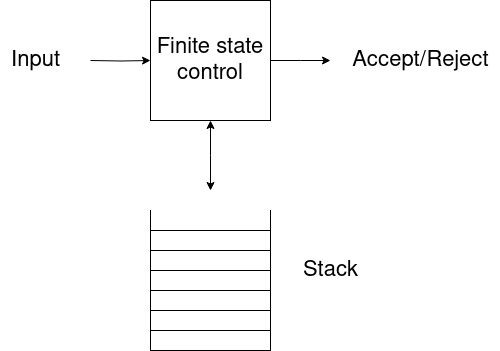
\includegraphics[scale = 0.4]{media/pda.png}
	\centering
	\caption{PDA, automa con pila}
\end{figure}
Esempio: Consideriamo il linguaggio palindromo: 
\[ L_{wwr} = \{ ww^R : w \in \{0,1\}^*\}\]
Una PDA per $L_{wwr}$ ha 3 stati: 
\begin{enumerate}
  \item In $q_0$ si presume l'input non sia esaurito, quindi leggo 1 alla volta tutti i simboli di input e li accumulo nello stack.
  \item Scommettiamo di aver trovato la sequenza corretta, quindi passiamo in $q_1$ ma continuando a leggere input
  \item Confronta la cima della pila con il simbolo in $q_1$, se sono uguali consumiamo l'elemento, altrimenti il ramo muore
  \item Se lo stack è vuoto passiamo in $q_2$
\end{enumerate}

\subsection{Definizione formale PDA}
Un PDA è una tupla di 7:
\[ P = (Q,\Sigma, \Gamma, \delta, q_0, Z_0,F)\]
dove 
\begin{itemize}
  \item Q è un insiemi di stati finiti
  \item $\Sigma$ è un alfabeto finito di input
  \item $\Gamma$ è un alfabeto finito di pila
  \item ($\delta$ è una funzione di transizione da $Q\times(\Sigma \cup \{\epsilon\}) \times \Gamma$ a sottoinsieme di $Q \times \Gamma^*$ - definizione del prof, poco chiara)
    \\ $\delta$ è un funzione di transizione che prende 3 input $(q,a, X)$ dove: 
    \begin{itemize}
      \item q è uno stato in Q
      \item a è un simbolo in $\Sigma$ oppure la $\epsilon$, NB $\epsilon$ non fa parte dell'input
      \item X è un simbolo in $\Gamma$, ovvero è un simbolo \textbf{sullo stack}
    \end{itemize}
    L'output di $\sigma$ è una coppia $(p, \gamma)$, dove p è uno stato e $\gamma$ è una nuova stringa che rimpiazza $X$ sullo stack. 
    Se $\gamma = \epsilon$ $X$ viene eliminato, se $\gamma = X$ non cambia nulla e se $\gamma = YZ$ allora $Y$ sostituisce $X$ e $Z$ viene aggiunto allo stack

  \item $q_0$ stato iniziale 
  \item $Z_0 \in \Gamma$ simbolo iniziale per la pila
  \item $F \subseteq Q$ è l'insieme degli stati di accettazione
\end{itemize}

\newpage
Prendiamo come esempio il PDA di $L_{wwr}$: 
\[P=(\{q_0, q_1, q_2\}, \{0,1\}, \{Z_0, 0, 1\}, \delta, q_0, Z_0, \{ q_2 \}\]

\begin{figure}[ht]
	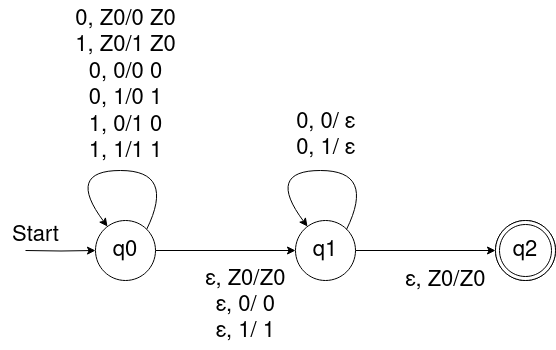
\includegraphics[scale = 0.4]{media/pda_diag.png}
	\centering
\end{figure}

dove $\delta$ è definita dalle seguenti regole: 
\begin{enumerate}
  \item $\delta(q_0,0,Z_0)$ = $\{(q_0, 0Z_0)\}$ 
        $\delta(q_0,1,Z_0)$ = $\{(q_0, 1Z_0)\}$ 
        una di queste regole è applicata all'inizio, l'input viene inserito lasciando $Z_0$ come indice del fondo.
  \item 
        $\delta(q_0,0,0)$ = $\{(q_0, 00)\}$,
        $\delta(q_0,0,1)$ = $\{(q_0, 01)\}$,
        \\ $\delta(q_0,1,0)$ = $\{(q_0, 10)\}$,
        $\delta(q_0,1,1)$ = $\{(q_0, 11)\}$
        \\ leggo un input, lo salvo nello stack e continuo a leggere 
  \item 
        $\delta(q_0,\epsilon,Z_0)$ = $\{(q_1, Z_0)\}$,
        \\ $\delta(q_0,\epsilon,0)$ = $\{(q_1, 0)\}$ 
        \\ $\delta(q_0,\epsilon,1)$ = $\{(q_1, 1)\}$ 
        \\ passiamo da $q_0$ a $q_1$ lasciando intantto lo stack
  \item 
        $\delta(q_1,0,0)$ = $\{(q_1, \epsilon)\}$,
        \\ $\delta(q_1,1,1)$ = $\{(q_1, \epsilon)\}$
        \\ rimaniamo su $q_1$ ma eliminiamo un membro dallo stack, se sono uguali
  \item 
        $\delta(q_1,\epsilon,Z_0)$ = $\{(q_2, Z_0)\}$
        se non ho niente nello stack, passo alla soluzione accettante

\end{enumerate}

\newpage
\subsection{Descrizioni istantanee}
Un PDA passa da una configurazione all'altra consumando un simbolo in input oppure la cima della stack.
\\ Possiamo rappresentare una configurazione tramite \emph{descrizioni istantanee} (ID) che sono un tupla $(q, w,\gamma)$ dove: q è lo stato, w è l'input rimanente e $\gamma$ è il contenuto della pila. 
\\ Sia $P=(Q,\Sigma, \Gamma, \delta, q_0, Z_0, F)$ un PDA, allora $\forall w \in \Sigma^*, \beta \in \Gamma^*: (p,\alpha) \in \delta(q,a,X) \Rightarrow (q, aw, X\beta) \vdash (p,w,\alpha, \beta)$
\\ Il simbolo $\vdash$ significa "deduzione logica", mentre definiamo $\overset{*}{\vdash}$ come la chiusura transitiva di $\vdash$ 

	\begin{figure}[ht]
		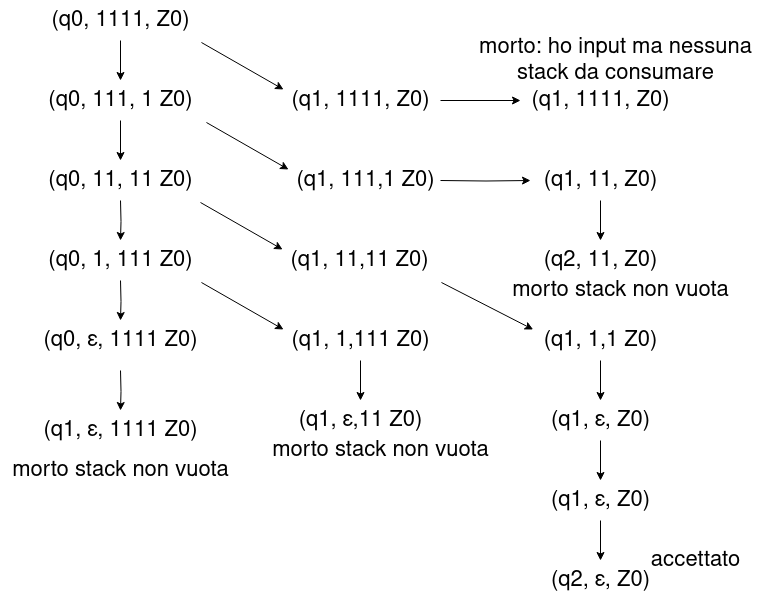
\includegraphics[scale = 0.5]{media/diagramma_pda.png}
		\centering
    \caption{Diagramma PDA}
	\end{figure}

\subsection{Accettazione per stato finale} 
Sia $P=(Q,\Sigma, \Gamma, \delta, q_0, Z_0, F)$ un PDA, il \emph{linguaggio accettato} da P per stato finale è: 
\[L(P)=\{w:(q_0,w,Z_0) \overset{*}{\vdash}(q,\epsilon,\alpha, q \in F)\}\]
In altre parole una volta che $w$ è in uno stato accettante il contenuto della pila è irrilevante

\subsection{Accettazione per pila vuota} 
Sia $P=(Q,\Sigma, \Gamma, \delta, q_0, Z_0, F)$ un PDA, il \emph{linguaggio accettato} da P per pila vuota è: 
\[N(P)=\{w:(q_0,w,Z_0) \overset{*}{\vdash}(q,\epsilon,\epsilon)\}\]
NB $q$ è un generico stato, dunque $N(P)$ è degli input $w$ che svuotano la stack

\newpage
\subsection{Da stack vuota a stato finale} 
Dimostriamo ora che per pila vuota o per stato finale sono linguaggi equivalenti. 
\\ \textbf{Teorema}: Se $L=N(P_N)$ per un PDA $P=(Q,\Sigma, \Gamma, \delta, q_0, Z_0)$ allora $\exists$ PDA $P_F$ tale che $L=N(P_F)$.
\\ \textbf{A parole}: L'idea è avere un simbolo nuovo $X_0$ che specifica quando arrivano allo stato finale sia $P_F$ che $P_N$. $p_0$ ci server per inserire il primo simbolo nello stack ed andare in $q_0$. Andiamo in $p_F$ quando $P_N$ svuota la stack. 
\begin{figure}[ht]
	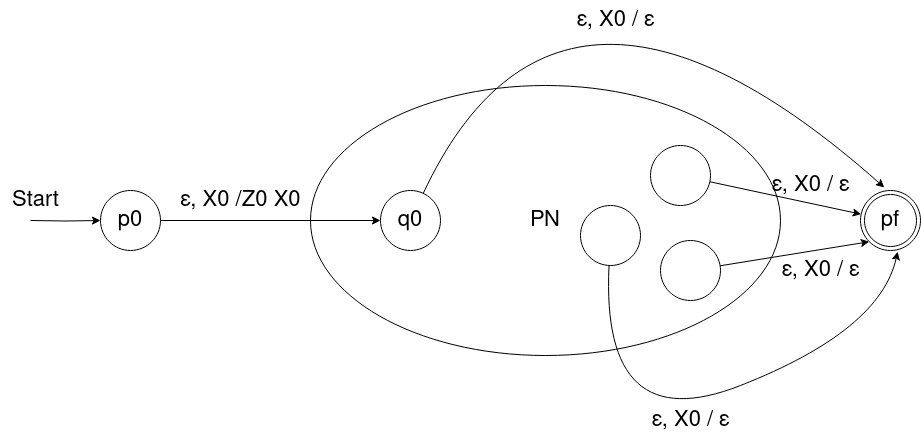
\includegraphics[scale = 0.4]{media/PNPF.png}
	\centering
\end{figure}
\\
\textbf{Dimostrazione} Sia: 
\[P_F = \{Q \cup \{p_0, p_f\}, \Sigma, \Gamma \cup \{ X_0\}, \delta_F, p_0, X_0, \{p_f\}\}\]
dove $\delta$ è definita come: 
\begin{enumerate}
  \item $\delta(p_0,\epsilon, X_0)=\{(q_0,Z_0, X_0)\}$
    transazione spontanea da $P_F$ a $P_N$
  \item $\forall q \in Q,a \in \Sigma \cup \{\epsilon\}, Y \in \Gamma: \delta_F(q,a,Y) =\delta_N(q,a,Y)$
  \item $\delta_F(q,a,Y)$ contiene $(p_j, \epsilon)$ per ogni $q$ in $Q$
\end{enumerate}

\newpage
Consideriamo un automa \emph{if} \emph{else} in C, dobbiamo leggere tanti if quanti else quindi usiamo Z per contare la differenza tra i 2 simboli.

\begin{figure}[ht]
	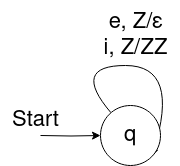
\includegraphics[scale = 0.4]{media/if_else.png}
	\centering
\end{figure}

Leggendo i inseriamo una Z, leggendo e rimuoviamo una Z.Formalmente: 
\[ P_N = (\{q\}, \{i,e\}, \{Z\}, \delta_N,q,Z) \]
dove $\delta$: 
\begin{enumerate}
  \item $\delta(q,i,Z) = \{(q,ZZ)\}$ leggo i aggiungo Z 
  \item $\delta(q,e,Z) = \{(q,\epsilon)\}$ leggo e rimuovo Z
\end{enumerate}
A partire da $P_N$ costruiamo $P_F$:
\[ P_F = (\{p,q,r\}, \{i,e\}, \{Z,X_0\}, \delta_F,p,X_0, \{r\}) \]
dove $\delta$:
\begin{enumerate}
  \item $\delta_F(p,\epsilon, X_0) = \{(q,ZX_0)\}$ simulo lettura primo simbolo, $X_0$ va in fondo allo stack
  \item $\delta_F(q, i, Z) = \{(q,ZZ)\}$ leggo i aggiungo Z
  \item $\delta_F(q, e, Z) = \{(q,\epsilon)\}$ leggo e rimuovo z
  \item $\delta_F(q, \epsilon, X_0) = \{(r,\epsilon)\}$ $P_F$ accetta quando $P_N$ si svuota
\end{enumerate}

\begin{figure}[ht]
	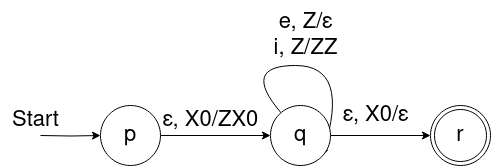
\includegraphics[scale = 0.4]{media/if_else_pf.png}
	\centering
  \caption{Diagramma P\textsubscript{F}}
\end{figure}

\subsection{Da stato finale a pila vuota}
Facciamo il percorso inverso $P_F \rightarrow P_N$. Si aggiunge un $\epsilon$-transizione da ogni stato accettante di $P_F$ a un nuovo stato p. Quando siamo in p, consumo lo stack senza leggere input. 
\\ Per evitare di svuotare lo stack per stringhe non valide uso $X_0$ come indicatore di fondo. Il nuovo stato $p_0$ serve solo ad arrivare allo stato iniziale $q_0$ e mettere $X_0$ in fondo allo stack. 
\\ \textbf{Teorema}: Se $L=N(P_F)$ per un PDA $P_F=(Q,\Sigma, \Gamma, \delta_F, q_0, Z_0, F)$ allora $\exists$ PDA $P_N$ tale che $L=N(P_N)$.
\\ \textbf{Dimostrazione}: 
\[ P_N = (Q \cup \{p_0, p\}, \Sigma,\Gamma \cup \{X_0\}, \delta_N,p_0,X_0) \]
dove $\delta_N$ è:
\begin{enumerate}
  \item $\delta_N(p,\epsilon, X_0) = \{(q,ZX_0)\}$ simulo lettura primo simbolo, $X_0$ va in fondo allo stack
  \item $\forall \; q$ in $Q$, $a$ in $\Sigma$ e ogni $Y$ in $\Gamma$: $\delta_N(q,a,Y)$ contiene tutte le coppie  in $\delta_F(q,a,Y)$. Ovvero $P_N$ simula $P_F$.
  \item $\forall \; q$ in $F$ e ogni $Y$ in $\Gamma$: $\delta(q,a,Y)$ contiene $(p,\epsilon)$. Ogni volta che $P_F$ accetta $P_N$ può svuotare lo stack
  \item $\forall \; Y$ in $\Gamma$: $\delta(q,a,Y) = \{p, \epsilon\}$ quando arrivo a $p$, quindi $P_F$ ha accettato, $P_N$ svuota lo stack senza leggere input
\end{enumerate}

\begin{figure}[ht]
  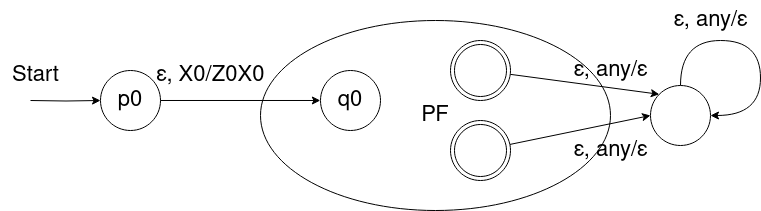
\includegraphics[scale = 0.4]{media/cfg_pda.png}
  \centering
\end{figure}

\newpage
\subsection{Equivalenza tra PDA e CFG} 
Un linguaggio è
generato da una CFG
se e solo se è
accettato da un PDA per pila vuota
se e solo se è
accettato da un PDA per stato finale

\subsection{Da CFG a PDA}
Data una CFG costruiamo una PDA che simula la derivazione a sinistra. Ogni espressione non terminale si può scrivere come $xA\alpha$, dove $A$ è la variabile più a sinistra, $x$ sono gli simboli terminali a sinistra di $A$ e $\alpha$ sono le variabili alla destra di $A$.
\\ 
Chiamiamo $A\alpha$ la coda della forma/espressione. Una coda di terminali è da considerarsi $\epsilon$. Dobbiamo simulare un PDA, dove accettiamo una stringa terminale $w$. La coda di $xA\alpha$ compare sullo stack con A in cima, $x$ è quello che consumiamo per aggiungere una stack, $w=xy$.
\\ Quindi data la transazione $(q,y,A\alpha)$, che rappresenta $xA\alpha$, l'automa sceglie di espandere $A \rightarrow \beta$. $\beta$ va in cima allo stack entrando nella ID $(q,y,\beta \alpha)$, il PDA ha un unico stato $q$.
\\ Non è detto però che $\beta$ sia terminale, e potrebbe avere dei terminali che lo precedono, quindi dobbiamo eliminare ogni terminale all'inizio di $\beta \alpha$. Confronto i terminali con i successi input per verificare correttezza, altrimenti il processo muore. 
\\ Nel caso in cui tutto vada bene, lo stack è vuoto e abbiamo la $w$ corretta. 
\\ Formalmente: Sia $G=(V,T,Q,S)$ una CFG, costruiamo il PDA $P$ che accetta $L(G)$ per stack vuoto: 
\[ P = (\{q\},T,V \cup T, \delta, q, S) \]
dove $\delta$ è definita come segue 
\[\delta(q,\epsilon,A) = \{(q,\beta): A \rightarrow \beta \in Q\}\]
per ogni terminale a, $\delta(q,a,a) = \{(q, \epsilon)\}$
\\ \textbf{Esempio:} 
\\ Considero la grammatica $S \rightarrow \epsilon|SS|iS|iSe$. Il PDA corrispondente è: 
\[ P = (\{q\}, \{i,e\}, \{S,i,e\},\delta,q,S)\]
dove $\delta(q,\epsilon,S)=\{(q,\epsilon),(q,SS),(q,iS),(q,iSe)\}, \delta(q,i,i)=\{(q,\epsilon)\} 
\\ \delta(q,e,e)=\{(q,\epsilon)\}$.

\subsection{Da PDA a CFG}
Per ogni PDA $P$ possiamo costruire un CFG $G$ il cui linguaggio coincide con quello accettato dallo stack vuoto di $P$. Dobbiamo prendere atto del momento più importante di una PDA, ovvero quando viene fatto il pop di un elemento dello stack, perché è cambiato lo stato. Nel nostro caso server tenere traccia dello stato passato. Ogni stato che cambia "scendo" nello stack.

\begin{figure}[ht]
	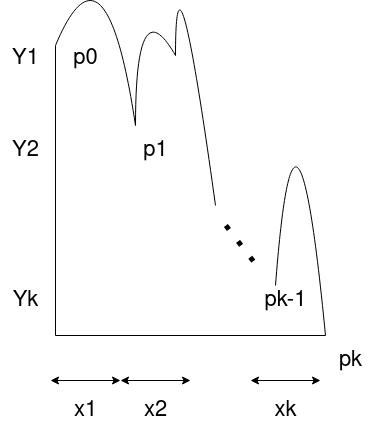
\includegraphics[scale = 0.4]{media/grafico_pda.png}
	\centering
\end{figure}
Nel grafico si può notare che ogni eliminazione $Y_1,Y_2,...,Y_k$ coincide con la lettura di un input $x$. Non importa quanti passaggi siano stati fatti, qua viene visto lo step finale, quando $Y$ esce.
\\ Inoltre viene visto anche il passaggio di stato, che anche esso coincide con l'eliminazione.
\\ Per costruire una CFG a partire dal PDA usiamo variabile che rappresentano un "evento" con due parti: 
\begin{enumerate}
  \item l'eliminazione definitiva dallo stack di $X$
  \item il passaggio da $p$ a $q$, dopo che scambio $X$ con $\epsilon$ sullo stack
\end{enumerate}
Questa variabile la rappresentiamo come $[pXq]$. 
\\ \textbf{Formalmente}: Sia $P=(Q,\Sigma,\Gamma, \delta,q_0,Z_0)$ un PDA. \\ Definiamo $G=(V,\Sigma,R,S)$ con:
\begin{itemize}
  \item $V=\{[pXq]:\{p,q\} \subseteq Q,X \in \Gamma\} \cup \{S\}$ ovvero V contiene il simbolo iniziale $S$ e tutti i simboli in $Q$ e in $\Gamma$
  \item $R= \{S \rightarrow [q_0 Z_0 p]:p \in Q \} \cup$ \\ $\{q X r_k] \rightarrow a[r Y_1 r_1]...[r_{k-1} Y_k r_k]:$
  \\ $a \in \Sigma \cup \{\epsilon\}$,
  \\ $\{r_1,...,r_k\} \subseteq Q$, 
  \\ $(r,Y_1 Y_2...Y_k) \in \delta(q,a,X)\}$
  \begin{itemize}
      \item $[q_0 Z_0 p]$ genera tutte le stringhe $w$ e passa dallo stato $q_0$ a $p$. Al termine dell'operazione lo stack P sarà svuotato
      \item $\{q X r_k] \rightarrow a[r Y_1 r_1]...[r_{k-1} Y_k r_k]:$ è una produzione che indica il passaggio $q$ a $r_k$ e il susseguirsi di passaggi per arrivarci. Al primo passaggio leggo l'input $a$ e itero k volte finché non ho eliminato Y. $a$ può essere $\epsilon$
        \item se k=0 allora $Y_1 Y_2 ... Y_k = \epsilon$ e $r_k = r$
  \end{itemize}
\end{itemize}
\textbf{Esempio}: Convertiamo

\begin{figure}[ht]
	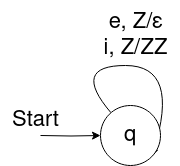
\includegraphics[scale = 0.4]{media/if_else.png}
	\centering
\end{figure}
\[ P_N = (\{q\}, \{i,e\}, \{Z\}, \delta_N,q,Z) \]
dove 
\begin{itemize}
  \item $\delta(q,i,Z) = \{(q,ZZ)\}$ 
  \item $\delta(q,e,Z) = \{(q,\epsilon)\}$ 
\end{itemize}
in una grammatica 
\[G=(V,\{i,e\},R,S)\]
dove 
\begin{itemize}
  \item $V=\{[qZq],S\}$
  \item $R=\{S \rightarrow [qZq],[qZq] \rightarrow i[qZq[qZq], [qZq] \rightarrow e \}$
\end{itemize}
Per semplicità $[qZq]=A$ quindi $S \rightarrow A$ e $A=iAA|e$

\textbf{Esempio}: Convertiamo 
\[ P = \{p,q\}, \{0,1\},\{X,Z_0\},\delta, q, Z_0) \]
dove $\delta$ è data da: 
\begin{enumerate}
  \item $\delta(q,1,Z_0) = \{(q,XZ_0)\}$
  \item $\delta(q,1,X) = \{(q,XX)\}$
  \item $\delta(q,0,X) = \{(p,X)\}$
  \item $\delta(q,\epsilon,X) = \{(q,\epsilon)\}$
  \item $\delta(p,1,X) = \{(p,\epsilon)\}$
  \item $\delta(p,0,Z_0) = \{(q,Z_0)\}$
\end{enumerate}
in una CFG.
\\ Otteniamo $G=(V,\{0,1\},R,S$, dove 
\[ V = \{[qZ_0q],[pZ_0q],[qZ_0p],[pZ_0p], [qXq],[pXq],[qXp],[pXp],\} \]
e le produzioni in R 
\[ S \rightarrow [q Z_0 q] [qZ_0p]\]
Dalla transizione (1) $\delta(q,1,Z_0) = \{(q,XZ_0)\}$ si ha:
\\ $[q Z_0 q] \rightarrow 1[qXq][qZ_0 q]$
\\ $[q Z_0 q] \rightarrow 1[qXp][pZ_0 q]$
\\ $[q Z_0 p] \rightarrow 1[qXq][qZ_0 p]$
\\ $[q Z_0 p] \rightarrow 1[qXp][pZ_0 p]$
\vspace{2mm}
\\ Dalla transizione (2) $\delta(q,1,X) = \{(q,XX)\}$
\\ $[qXq] \rightarrow 1[qXq][qXq]$
\\ $[qXq] \rightarrow 1[qXp][pXq]$
\\ $[qXp] \rightarrow 1[qXq][qXp]$
\\ $[qXp] \rightarrow 1[qXp][pXp]$
\vspace{2mm}
\\ Dalla transizione (3) $\delta(q,0,X) = \{(p,X)\}$
\\ $[qXq] \rightarrow 0[pXq]$
\\ $[qXp] \rightarrow 0[pXp]$
\vspace{2mm}
\\ Dalla transizione (4) $\delta(q,\epsilon,X) = \{(q,\epsilon)\}$
\\ $[qXq] \rightarrow \epsilon$
\vspace{2mm}
\\ Dalla transizione (5) $\delta(p,1,X) = \{(p,\epsilon)\}$
\\ $[pXp] \rightarrow 1$
\vspace{2mm}
\\ Dalla transizione (6) $\delta(p,0,Z_0) = \{(q,Z_0)\}$
\\ $[pZ_0 q] \rightarrow 0[qZ_0 q]$
\\ $[pZ_0 p] \rightarrow 0[qZ_0 p]$


\section{PDA deterministici}
I PDA deterministici sono quelli usati per i parser, sono un sotto caso utile per noi.
\\ 
Un PDA deterministico non deve avere mosse alternative, se $\delta(q,a,X)$ ha più di una coppia sicuramente non è deterministico. Questo però non è sufficiente però, perché potresti avere due prodotti diversi e bisogna scegliere.
\\ Definiamo quindi un PDA $P=(Q, \Sigma, \Gamma, \delta, q_0, Z_0, F)$ deterministico se e solo se: 
\begin{enumerate}
  \item $\delta(q,a,X)$ ha al massimo un elemento $\forall q \in Q, a \in \Sigma, X \in \Gamma$
  \item Se $\delta(q,a,X)$ non è vuoto per un $a \in \Sigma$ allora $\delta(q,\epsilon,X)$ deve essere vuoto
\end{enumerate}

\begin{figure}[ht]
	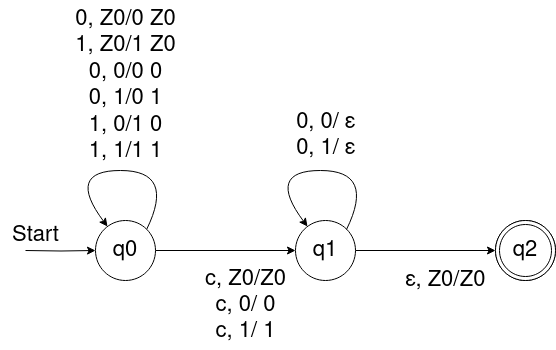
\includegraphics[scale = 0.4]{media/pda_det.png}
	\centering
  \caption{Esempio di PDA deterministico (DPDA)}
\end{figure}

\newpage
\subsection{DPA che accettano per stato finale} 
Regex $\subset$ L(DPDA) $\subset$ CFL.
\\ \textbf{Teorema} Se L è regolare allora L=L(P) per un qualsiasi DPDA P.
\\ \textbf{Prova}: Dato che L è regolare $\exists$ DFA $A$ tale che L=L(A)
\[A=(Q,\Sigma, \delta_A, q_0, F)\]
definiamo il DPDA
\[P=(Q,\Sigma,\{Z_0\},\delta_P,q_0,Z_0,F)\]
dove
\[\sigma_P(q,a,Z_0) = \{(\delta_A(q,a),Z_0\}\]
$\forall \; p,q \in Q$ e $a \in \Sigma$
\\ applichiamo un induzione su $|w|$
\[(q_0,w,Z_0) \overset{*}{\vdash} (p,\epsilon, Z_0) \iff \circumdelta(q_0,w)=p\]

\subsection{DPDA che accettano per la pila vuota}
Si usa la \textbf{proprietà del prefisso}: un linguaggio ha la proprietà del prefisso se NON esistono due stringhe uguali una che è il prefisso dell'altra. 
\\ $L_{pal}$ ha la proprietà del prefisso
\\ $\{0\}^*$ non ha la proprietà del prefisso
\\ \textbf{Teorema} L è N(P) per un qualche DPDA P se e solo se L ha la proprietà del prefisso e L è $L(P')$ per qualche DPDA $P'$

\subsection{DPDA e non ambiguità}
L(DPDA) non per forza coincide con CFL non ambigue, viceversa invece è vero. 
\begin{theorem}
Se $L=N(P)$ per qualche DPDA P, allora L ha una grammatica non ambigua 
\label{dpda1}
\end{theorem}
\textbf{Dimostrazione} stessa dimostrazione che fai da PDA a CFG, solo che parti con un DPDA
\vspace{2mm}
\\ L'enunciato può essere rafforzato 
\begin{theorem}
 Se $L=L(P)$ per qualche DPDA P, allora L ha una grammatica non ambigua 
 \label{dpda2}
\end{theorem}
\textbf{Dimostrazione}
\\ Sia \$ un simbolo non presente in $L$, e sia $L'=L\$$. In altri termini L' sono le stringhe L seguite da \$.
Dal Teorema. \ref{dpda1} L' ha la proprietà di prefisso.
Dal Teorema. \ref{dpda2} esiste una grammatica $G'$ che genera un linguaggio $N(P')$ che è $L'$.
\\ Costruiamo quindi una grammatica $G$ tale che $L(G)=L$, dobbiamo solo togliere \$ dalla fine delle stringhe, così che $G'$ coincida con $G$. Introduciamo \$ in $G$
\[ \$ \rightarrow \epsilon \]
Visto che $L(G')=L'$ consegue che $L(G)=L$. $G$ non è ambigua.

\section{Proprietà di CFG}
Elenco delle proprietà: 
\begin{itemize}
  \item \emph{Semplificazione} di una CFG. Una CFL ha una grammatica in forma speciale
  \item \emph{Pumping Lemma} per CFG, simile alle regex
  \item \emph{Proprietà di chiusura}.
  \item \emph{Proprietà di decisione}. Verifichiamo l'appartenenza e l'essere vuoto 
\end{itemize}

\subsection{Forma normale di Chomsky}
Ogni CFL (senza $\epsilon$) è generato da una CFG dove tutte le forme sono 
\[A \rightarrow BC, A \rightarrow a\]
dove $A,B,C$ sono variabili, mentre $a$ è un terminale. Questa è detta forma di Chomsky e per ottenerla dobbiamo pulire la grammatica: 
\begin{itemize}
  \item Eliminare i \emph{simboli inutili}, ovvero ogni simbolo che non appartiene a $S \overset{*}\Rightarrow w$
  \item Eliminare le \emph{produzioni} $\epsilon$, dalla forma $A \rightarrow \epsilon$
  \item Eliminare le \emph{produzioni unità} ovvero le produzioni $A \rightarrow B$
\end{itemize}

\subsection{Eliminazione di simboli inutili} 
Un simbolo $X$ è \emph{utile} per una grammatica $G=(V,T,P,S)$ se esiste una derivazione 
\[ S \xRightarrow[G]{*} \alpha X \beta \xRightarrow[G]{*} w\]
per una stringa $w \in T^*$. Possiamo eliminare i simboli inutili senza cambiare il significato della grammatica. Un simbolo utile deve avere 2 caratteristiche: 
\begin{enumerate}
  \item $X$ è un \emph{generatore} se esiste una stringa w tale che $X \xRightarrow[]{*} w$. Ogni terminale è un generatore di se stesso in 0 passi
  \item $X$ è \emph{raggiungibile} se esiste una derivazione $S \xRightarrow[]{*} \alpha X \beta$ per qualche $\{\alpha, \beta\} \subseteq (V \cup T)^*$
\end{enumerate}
Un simbolo deve essere sia raggiungibile che generatore, eliminando prima i non generatori e poi i non raggiungibili abbiamo una grammatica solo di simboli utili.
\\ \textbf{Esempio}: Consideriamo la grammatica 
\[ S \rightarrow AB | a \]
\[ A \rightarrow b \]
A genera b, S genera A, B non è un simbolo generatore. Eliminando B: 
\[ S \rightarrow a \]
\[ A \rightarrow b \]
Adesso solo $a$ è raggiungibile quindi 
\[ S \rightarrow a \]
che è la nostra grammatica iniziale
\\ 
NB se elimino prima i simboli non raggiungibili non cambia nulla, tutto è raggiungibile
\[ S \rightarrow AB | a \]
\[ A \rightarrow b \]
ora elimino $B$ 
\[ S \rightarrow a \]
\[ A \rightarrow b \]
e ho una grammatica con simboli inutili

\subsection{Eliminazione delle produzioni epsilon}
Se L è un CFL, allora L \{$\epsilon\}$ ha una grammatica priva di produzioni $\epsilon$.
\\ La variabile A è annullabile se $A \xRightarrow[]{*}\epsilon$
\\ Sia a annullabile, rimpiazzo 
\[ B \rightarrow \alpha A \beta\]
\\ con
\[ B \rightarrow \alpha \beta\]
indico con n(G) l'insieme dei simboli annullabili della grammatica $G=(V,T,P,S)$.
\\ \textbf{Esempio} Sia la grammatica
\[ S \rightarrow AB, A \rightarrow aAA|\epsilon, B \rightarrow bBB|\epsilon\]
Abbiamo $n(G)=\{A,B,S\}$, la prima regola diventa 
\[ S \rightarrow AB| A |B \]
la seconda regola diventa
\[ A \rightarrow aAA| aA | aA |a \]
la terza regola diventa
\[ B \rightarrow bBB| bB | bB |b \]
La nuova grammatica sarà: 
\[ S \rightarrow AB| A |B 
A \rightarrow aAA| aA |a
B \rightarrow bBB| bB |b
\]

\subsection{Eliminazione produzioni unità}
\[A \rightarrow B \]
è una produzione unità nel caso in cui A e B siano variabili. Le produzioni variabili sono eliminabili.
\\ Data la grammatica 
\\ $ E \rightarrow T | E + T$
\\ $ T \rightarrow F | T * F$
\\ $ F \rightarrow I | (E) $
\\ $ I \rightarrow a | b | Ia | Ib | I0 | I1 $
\\ le produzioni unità sono $E \rightarrow T, T \rightarrow F, F \rightarrow I$ 
\\ Considero la produzione $E \rightarrow T$ e la espando 
\[ E \rightarrow F, E \rightarrow T * F \]
poi espando $E \rightarrow F$
\[ E \rightarrow I, (E), T * F \]
Infine espando $E \rightarrow I$
\[ E \rightarrow a | b| Ia |Ib|I0|I1|(E)|T*F\]
lo stesso applico lo stesso procedimento con $T \rightarrow F$ e $F \rightarrow I$: 
\[ T \rightarrow a | b| Ia |Ib|I0|I1|(E)\]
\[ F \rightarrow a | b| Ia |Ib|I0|I1\]
la nuova grammatica sarà 
\\ $ E \rightarrow a | b | Ia | Ib | I0 | I1  | (E) | T*F | E+T $
\\ $ T \rightarrow a | b | Ia | Ib | I0 | I1  | (E) | T * F$
\\ $ F \rightarrow a | b | Ia | Ib | I0 | I1  | (E) $
\\ $ I \rightarrow a | b | Ia | Ib | I0 | I1  $
\\ Questo procedimento non funziona nel caso in cui ci siano dei cicli. Se trovo un unità già espansa la rimuovo.
\vspace{2mm}
\\ \textbf{Esempio} Si consideri la grammatica
\\ $ A \rightarrow B | a$
\\ $ B \rightarrow C | b$
\\ $ C \rightarrow A | c$
\\ Espando $ A \rightarrow B$
\\ Da $ A \rightarrow B $ ottengo 
\[ A \rightarrow C | b \]
\\ Da $ A \rightarrow C $ ottengo 
\[ A \rightarrow A | c | b \]
\\ Da $ A \rightarrow A $ ottengo 
\[ A \rightarrow B \; a | c | b \]
Qui mi fermo perché tornei a fare le stesse produzioni, mi rimane:
\[ A \rightarrow a | c | b \]
eseguo per le altre 3 e la nuova grammatica risulta 
\[ A \rightarrow a | b | c \]
\[ B \rightarrow a | b | c \]
\[ C \rightarrow a | b | c \]

\subsection{Sommario} 
Per pulire una grammatica bisogna: 
\begin{enumerate}
  \item Eliminare le produzioni $\epsilon$
  \item Eliminare le produzioni unità
  \item Eliminare simboli inutili
\end{enumerate}
in quest'ordine

\subsection{Forma normale di Chomsky, CNF}
Ogni CNF non vuoto, senza $\epsilon$, ha una grammatica $G$ di simboli inutili nella seguente forma 
$A \rightarrow BC$ dove $\{A,B,C\} \subseteq V$ oppure
$A \rightarrow a$ dove $a\in T$ e $A \in V$.
\\ Per arrivare a questa forma bisogna: 
\begin{itemize}
  \item Pulire la grammatica 
  \item Modificare le produzioni con 2 o più simboli in modo che siano tutte variabili 
  \item Ridurre le produzioni con più di 2 simboli in catene da 2 simboli
\end{itemize}
Quindi per ogni terminale $a$ più lungo di 1 creo una nuova variabile $A \rightarrow a$.
Mentre per ogni regola 
\[ A \rightarrow B_1,B_2,...,B_k \]
$k \geq 3$ creo nuove variabili $C_1, C_2, ..., C_{k-2}$
\[ A \rightarrow B_1, C_1 \]
\[ C_1 \rightarrow B_2, C_2 \]
\[...\]
\[ C_{k-3} \rightarrow B_{k-2}, C_{k-2} \]
\[ C_{k-2} \rightarrow B_{k-1}, B_k \]
\textbf{Esempio}
Usiamo la grammatica 
\\ $E\rightarrow | E+F | T*F | (E) | b | Ia | Ib | I0 | I1   $
\\ $T\rightarrow (E) | T*F | a | b | Ia | Ib | I0 | I1$
\\ $F\rightarrow (E)| a | b | Ia | Ib | I0 | I1   $
\\ $I\rightarrow a | b | Ia | Ib | I0 | I1  $
\vspace{5mm}
\\ applichiamo il passo 2
\\ $A \rightarrow a, B \rightarrow b, Z \rightarrow 0, O \rightarrow 1 $
\\ $P \rightarrow +, M \rightarrow *, L \rightarrow (, R \rightarrow ) $
\vspace{5mm}
\\ otteniamo 
\\ $E\rightarrow EPF | TMF | LER | b | IA | IB | IZ | IO   $
\\ $T\rightarrow LER | TMF | a | b | IA | IB | IB | IO$
\\ $F\rightarrow LER | a | b | IA | IB | IZ | IO$
\\ $I\rightarrow a | b | IA | IB | IZ | IO $
\\ $A \rightarrow a, B \rightarrow b, Z \rightarrow 0, O \rightarrow 1 $
\\ $P \rightarrow +, M \rightarrow *, L \rightarrow (, R \rightarrow ) $
\vspace{5mm}
\\ Applichiamo il passo 3
\\ $E \rightarrow EPT$ diventa $E \rightarrow EC_1, C_1 \rightarrow PT$
\vspace{2mm}
\\ $E \rightarrow TMF, T \rightarrow TMF$ diventa $E \rightarrow TC_2,T \rightarrow TC_2, C_2 \rightarrow MF$
\vspace{2mm}
\\ $E \rightarrow LER, T \rightarrow LER, F \rightarrow LER$ diventa $E \rightarrow LC_3,T \rightarrow TC_3, F \rightarrow LC_3, C_3 \rightarrow ER$
\vspace{5mm}
\\ La grammatica finale diventa 
\\ $E\rightarrow EC_1 | TC_2 | LC_3 | b | IA | IB | IZ | IO   $
\\ $T\rightarrow LC_3 | TC_2 | a | b | IA | IB | IB | IO$
\\ $F\rightarrow LC_3 | a | b | IA | IB | IZ | IO$
\\ $I\rightarrow a | b | IA | IB | IZ | IO $
\\ $C_1 \rightarrow PT$, $C_2 \rightarrow MF$, $C_3 \rightarrow ER$
\\ $A \rightarrow a, B \rightarrow b, Z \rightarrow 0, O \rightarrow 1 $
\\ $P \rightarrow +, M \rightarrow *, L \rightarrow (, R \rightarrow ) $

\subsection{Pumping lemma per CFL}
\textbf{Pumping lemma per i linguaggi regolari}: per una stringa sufficiente lunga è possibile causare un ciclo e creare un infinità di stringhe che appartengono al linguaggio 
\\ \textbf{Pumping lemma per CFL}: per una stringa sufficiente lunga è possibile trovare due sottostringhe vicine che si possono iterare "in tandem". Posso iterare $i$ volte per trovare nuove stringhe appartenenti al linguaggio.
\\ \textbf{Formalmente}: 
\\ Sia L un CFL. Allora $\exists n \geq 1$ che soddisfa: ogni $z \in L: |z| \geq n$ è composto da 5 stringhe $z=uvwxz$ tali che: 
\begin{enumerate}
  \item $|vwx| \leq n$
  \item $|vx| > 0$
  \item $\forall i \geq 0, uv^i wx^i y \in L$
\end{enumerate}

\newpage
\import{}{esercizi}
\end{document}
